\documentclass[14pt]{extarticle}

\usepackage[table]{xcolor} % colored lines for tables
\usepackage[normalem]{ulem} % strike through text
\usepackage{amsmath,mathtools,amsfonts,amsthm,amssymb,hyperref}
\usepackage{parskip,geometry,latexsym,bookmark,mathtools,float,cancel}
\usepackage{minted,tcolorbox,bm}

\usepackage[mathscr]{euscript}
\let\euscr\mathscr
\let\mathscr\relax
\usepackage[scr]{rsfso}
\newcommand{\ps}{\mathscr{P}} % for the Power set P

\newtheorem{defn}{Definition}
\newtheorem{thm}{Theorem}
\newtheorem{claim}{Claim}
\newtheorem{lemma}{Lemma}

\newcommand{\dps}{\displaystyle}
\newcommand{\es}{\varnothing}
\newcommand{\fbl}{\underline{\hspace{1cm}}\,\,}
\newcommand{\R}{\mathbb{R}}
\newcommand{\Q}{\mathbb{Q}}
\newcommand{\Z}{\mathbb{Z}}
\newcommand{\from}{\leftarrow}
\newcommand{\true}{{\bf t}}
\newcommand{\false}{{\bf c}}
\newcommand{\bic}{\leftrightarrow}
\newcommand{\da}{\downarrow}
\newcommand{\fa}{\forall}
\newcommand{\te}{\exists}
\newcommand{\cy}{\color{cyan}}

\newcommand{\colsq}[1]{{\color{#1} $\blacksquare$}}

\newcommand{\base}[1]{{\cy #1}} % for log bases
\newcommand{\floor}[1]{{\left\lfloor#1\right\rfloor}}
\newcommand{\ceil}[1]{{\left\lceil#1\right\rceil}}
\newcommand\Ccancel[2][black]{\renewcommand\CancelColor{\color{#1}}\cancel{#2}}
\newcommand\Cbcancel[2][black]{\renewcommand\CancelColor{\color{#1}}\bcancel{#2}}

\renewcommand{\arraystretch}{1.2}

\hypersetup{colorlinks,allcolors=blue,linktoc=all}
\geometry{a4paper}
\geometry{margin=0.42in}

\title{Solutions to Chapter 8, Susanna Epp Discrete Math 5th Edition}

\author{https://github.com/spamegg1}

\begin{document}
\maketitle
\tableofcontents


\section{Exercise Set 8.1}

\subsection{Exercise 1}
As in Example 8.1.2, the {\bf congruence modulo 2} relation $E$ is defined from $\Z$ to $\Z$ as follows: For every 
ordered pair \((m, n) \in \Z \times \Z\), $m$ $E$ $n$ \(\iff m - n\) is even.

\subsubsection{(a)}
Is $0$ $E$ $0$? Is $5$ $E$ $2$? Is $(6, 6) \in E$? Is $(21, 7) \in E$?

\begin{proof}
$0$ $E$ $0$ because \(0 - 0 = 0 = 2 \cdot 0\), so \(2 \mid (0 - 0)\). $5$ $\Ccancel{E}$ $2$ because \(5 - 2 = 3\) and 
\(3 \neq 2k\) for any integer $k$, so \(2 \nmid (5 - 2)\). \((6, 6) \in E\) because \(6 - 6 = 0 = 2 \cdot 0\), so \(2 
\mid (6 - 6). (-1, 7) \in E\) because \(-1 - 7 = -8 = 2 \cdot (-4)\), so \(2 \mid (-1 - 7)\).
\end{proof}

\subsubsection{(b)}
Prove that for any even integer $n$, $n$ $E$ $0$.

\begin{proof}
Assume $n$ is even. By definition of even, $n=2k$ for some integer $k$. Then \(n - 0 = 2k - 0 = 2k\) is also even.
Therefore by definition of $E$, $n$ $E$ 0.
\end{proof}

\subsection{Exercise 2}
Prove that for all integers $m$ and $n$, $m - n$ is even if, and only if, both $m$ and $n$ are even or both $m$ and 
$n$ are odd.

\begin{proof}
\(\bm{\implies}\): Assume $m-n$ is even. {\it [We want to prove that both $m$ and $n$ are even or both $m$ and $n$ 
are odd.]} By definition of even, \(m - n = 2k\) for some integer $k$. There are 4 cases:

{\bf Case 1: both $m$ and $n$ are even:} Nothing to prove.

{\bf Case 2: both $m$ and $n$ are odd:} Nothing to prove.

{\bf Case 3: $m$ is even, $n$ is odd:} By definitions of even and odd, \(m=2k, n=2l+1\) for some integers $k,l$. 
So \(m-n = 2k-2l-1 = 2(k-l-1) + 1\) where \(k-l-1\) is an integer. So by definition of odd, \(m-n\) is odd, a 
contradiction. So this case is impossible.

{\bf Case 4: $m$ is odd, $n$ is even:} By definitions of even and odd, \(m=2k+1, n=2l\) for some integers $k,l$. 
So \(m-n = 2k+1-2l = 2(k-l) + 1\) where \(k-l\) is an integer. So by definition of odd, \(m-n\) is odd, a 
contradiction. So this case is impossible.

\(\bm{\impliedby}\): Assume both $m$ and $n$ are even or both $m$ and $n$ are odd. {\it [We want to prove that $m-n$ 
is even.]} There are 2 cases:

{\bf Case 1: both $m$ and $n$ are even:} By definition of even, \(m = 2k, n = 2l\) for some integers $k,l$. Then 
\(m-n = 2k-2l = 2(k-l)\) where $k-l$ is an integer. So by definition, $m-n$ is even.

{\bf Case 2: both $m$ and $n$ are odd:} By definition of even, \(m = 2k+1, n = 2l+1\) for some integers $k,l$. Then 
\(m-n = 2k+1-2l-1 = 2(k-l)\) where $k-l$ is an integer. So by definition, $m-n$ is even.
\end{proof}

\subsection{Exercise 3}
The congruence modulo 3 relation, $T$, is defined from $\Z$ to $\Z$ as follows: For all integers $m$ and $n$, $m$ $T$ 
$n$ \(\iff 3 \mid (m - n)\).

\subsubsection{(a)}
Is $10$ $T$ $1$? Is $1$ $T$ $10$? Is \((2, 2) \in T\)? Is \((8, 1) \in T\)?

\begin{proof}
10 $T$ 1 because \(10 - 1 = 9 = 3 \cdot 3\), and so \(3 \mid (10 - 1)\).

1 $T$ 10 because \(1 - 10 = -9 = 3 \cdot (-3)\), and so \(3 \mid (1 - 10)\).

2 $T$ 2 because \(2 - 2 = 0 = 3 \cdot 0\), and so \(3 \mid (2 - 2)\).

8 $\Ccancel{T}$ 1 because \(8 - 1 = 7 \neq 3k\), for any integer $k$. So \(3 \nmid (8 - 1)\).
\end{proof}

\subsubsection{(b)}
List five integers $n$ such that $n$ $T$ $0$.

\begin{proof}
One possible answer: 3, 6, 9, $-3$, $-6$
\end{proof}

\subsubsection{(c)}
List five integers $n$ such that $n$ $T$ 1.

\begin{proof}
One possible answer: 4, 7, 10, $-2$, $-5$
\end{proof}

\subsubsection{(d)}
List five integers $n$ such that $n$ $T$ $2$.

\begin{proof}
One possible answer: 5, 8, 11, $-1$, $-4$
\end{proof}

\subsubsection{(e)}
Make and prove a conjecture about which integers are related by $T$ to $0$, which integers are related by $T$ to 
1, and which integers are related by $T$ to 2.

All integers of the form \(3k + 1\), for some integer $k$, are related by $T$ to $1$.

\begin{proof}
All integers of the form \(3k\), for some integer $k$, are related by $T$ to 0.

All integers of the form \(3k+1\), for some integer $k$, are related by $T$ to 1.

All integers of the form \(3k+2\), for some integer $k$, are related by $T$ to 2.
\end{proof}

\subsection{Exercise 4}
Define a relation $P$ on $\Z$ as follows: For every ordered pair \((m, n) \in \Z \times \Z\), $m$ $P$ $n$ \(\iff\) $m$ 
and $n$ have a common prime factor.

\subsubsection{(a)}
Is 15 $P$ 25?

\begin{proof}
Yes, because 15 and 25 are both divisible by 5, which is prime.
\end{proof}

\subsubsection{(b)}
Is 22 $P$ 27?

\begin{proof}
No, because 22 and 27 have no common prime factor.
\end{proof}

\subsubsection{(c)}
Is 0 $P$ 5?

\begin{proof}
Yes, because 0 and 5 are both divisible by 5, which is prime.
\end{proof}

\subsubsection{(d)}
Is 8 $P$ 8?

\begin{proof}
Yes, because 8 and 8 are both divisible by 2, which is prime.
\end{proof}

\subsection{Exercise 5}
Let \(X = \{a, b, c\}\). Recall that \(\ps(X)\) is the power set of $X$. Define a relation {\bf S} on \(\ps(X)\) 
as follows: For all sets $A$ and $B$ in \(\ps(X)\), $A$ {\bf S} $B$ $\iff$ $A$ has the same number of elements as $B$.

\subsubsection{(a)}
Is \(\{a, b\}\) {\bf S} \(\{b, c\}\)?

\begin{proof}
Yes, because both \(\{a, b\}\) and \(\{b, c\}\) have two elements.
\end{proof}

\subsubsection{(b)}
Is \(\{a\}\) {\bf S} \(\{a,b\}\)?

\begin{proof}
No, one has 1 element, the other has 2 elements.
\end{proof}

\subsubsection{(c)}
Is \(\{c\}\) {\bf S} \(\{b\}\)?

\begin{proof}
Yes, because both \(\{c\}\) and \(\{b\}\) have one element.
\end{proof}

\subsection{Exercise 6}
Let \(X = \{a, b, c\}\). Define a relation {\bf J} on \(\ps(X)\) as follows: For all sets $A$ and $B$ in $\ps(X)$,
$A$ {\bf J} $B$ $\iff$ \(A \cap B \neq \es\).

\subsubsection{(a)}
Is $\{a\}$ {\bf J} $\{c\}$?

\begin{proof}
No, because \(\{a\} \cap \{c\} = \es\).
\end{proof}

\subsubsection{(b)}
Is $\{a, b\}$ {\bf J} $\{b, c\}$?

\begin{proof}
Yes, because \(\{a,b\} \cap \{b,c\} = \{b\} \neq \es\).
\end{proof}

\subsubsection{(c)}
Is $\{a, b\}$ {\bf J} $\{a, b, c\}$?

\begin{proof}
Yes, because \(\{a,b\} \cap \{a,b,c\} = \{a,b\} \neq \es\).
\end{proof}

\subsection{Exercise 7}
Define a relation $R$ on $\Z$ as follows: For all integers $m$ and $n$, $m$ $R$ $n$ $\iff$ \(5 \mid (m^2 - n^2)\).

\subsubsection{(a)}
Is 1 $R$ $(-9)$?

\begin{proof}
Yes. 1 $R$ \((-9) \iff 5 \mid (1^2 - (-9)^2)\). But \(1^2 - (-9)^2 = 1 - 81 = -80\), and \(5 \mid (-80)\) because 
\(-80 = 5 \cdot (-16)\).
\end{proof}

\subsubsection{(b)}
Is 2 $R$ 13?

\begin{proof}
Yes, \(2^2 - (13)^2 = 4 - 169 = -165 = 5 \cdot (-33)\). So \(5 \mid 2^2 - (13)^2\).
\end{proof}

\subsubsection{(c)}
Is 2 $R$ $(-8)$?

\begin{proof}
Yes, \(2^2 - (-8)^2 = 4 - 64 = -60 = 5 \cdot (-12)\). So \(5 \mid 2^2 - (-8)^2\).
\end{proof}

\subsubsection{(d)}
Is $(-8)$ $R$ 2?

\begin{proof}
Yes, \((-8)^2 - 2^2 = 64 - 4 = 60 = 5 \cdot 12\). So \(5 \mid (-8)^2 - 2^2\).
\end{proof}

\subsection{Exercise 8}
Let $A$ be the set of all strings of $a$’s and $b$’s of length 4. Define a relation $R$ on $A$ as follows: For 
every \(s, t \in A\), $s$ $R$ $t$ $\iff$ $s$ has the same first two characters as $t$.

\subsubsection{(a)}
Is $abaa$ $R$ $abba$?

\begin{proof}
Yes, because both $abaa$ and $abba$ have the same first two characters $ab$.
\end{proof}

\subsubsection{(b)}
Is $aabb$ $R$ $bbaa$?

\begin{proof}
No, because the first two characters of $aabb$ are different from the first two characters of $bbaa$.
\end{proof}

\subsubsection{(c)}
Is $aaaa$ $R$ $aaab$?

\begin{proof}
Yes, because both $aaaa$ and $aaab$ have the same first two characters $aa$.
\end{proof}

\subsubsection{(d)}
Is $baaa$ $R$ $abaa$?

\begin{proof}
No, because the first two characters of $baaa$ are different from the first two characters of $abaa$.
\end{proof}

\subsection{Exercise 9}
Let $A$ be the set of all strings of 0’s, 1’s, and 2’s of length 4. Define a relation $R$ on $A$ as follows: For 
every \(s, t \in A\), $s$ $R$ $t$ $\iff$ the sum of the characters in $s$ equals the sum of the characters in $t$.

\subsubsection{(a)}
Is 0121 $R$ 2200?

\begin{proof}
Yes, because the sum of the characters in 0121 is 4 and the sum of the characters in 2200 is also 4.
\end{proof}

\subsubsection{(b)}
Is 1011 $R$ 2101?

\begin{proof}
No, because the sum of the characters in 1011 is 3, whereas the sum of the characters in 2101 is 4.
\end{proof}

\subsubsection{(c)}
Is 2212 $R$ 2121?

\begin{proof}
No, because the sum of the characters in 2212 is 7, whereas the sum of the characters in 2121 is 6.
\end{proof}

\subsubsection{(d)}
Is 1220 $R$ 2111?

\begin{proof}
Yes, because the sum of the characters in 1220 is 5 and the sum of the characters in 2111 is also 5.
\end{proof}

\subsection{Exercise 10}
Let \(A = \{3, 4, 5\}\) and \(B = \{4, 5, 6\}\) and let $R$ be the “less than” relation. That is, for every ordered 
pair \((x, y) \in A \times B, x \, R \, y \iff x < y\). State explicitly which ordered pairs are in $R$ and $R^{-1}$.

\begin{proof}
\(R = \{(3, 4), (3, 5), (3, 6), (4, 5), (4, 6), (5, 6)\}\)

\(R^{-1} = \{(4, 3), (5, 3), (6, 3), (5, 4), (6, 4), (6, 5)\}\)
\end{proof}

\subsection{Exercise 11}
Let \(A = \{3, 4, 5\}\) and \(B = \{4, 5, 6\}\) and let $S$ be the “divides” relation. That is, for every ordered pair 
\((x, y) \in A \times B, x \, S \, y \iff x \mid y\). State explicitly which ordered pairs are in $S$ and $S^{-1}$.

\begin{proof}
\(S = \{(3, 6), (4, 4), (5, 5)\}, S^{-1} = \{(6, 3), (4, 4), (5, 5)\}\)
\end{proof}

\subsection{Exercise 12}

\subsubsection{(a)}
Suppose a function \(F: X \to Y\) is one-to-one but not onto. Is \(F^{-1}\) (the inverse relation for $F$) a 
function? Explain your answer.

\begin{proof}
No. If \(F: X \to Y\) is not onto, then $F$ fails to be defined on all of $Y$. In other words, there is an element 
$y$ in $Y$ such that \((y, x) \notin F^{-1}\) for any \(x \in X\). Consequently, \(F^{-1}\) does not satisfy property 
(1) of the definition of function.
\end{proof}

\subsubsection{(b)}
Suppose a function \(F: X \to Y\) is onto but not one-to-one. Is \(F^{-1}\) (the inverse relation for $F$) a 
function? Explain your answer.

\begin{proof}
No. If \(F: X \to Y\) is not one-to-one, then $F$ for some $y$ in $Y$, there will be multiple potential values for 
\(F^{-1}(y)\). In other words, there is an element $y$ in $Y$ and elements \(x_1, x_2 \in X\) such that \((y, x_1) 
\in F^{-1}\) and \((y, x_2) \in F^{-1}\). Consequently, \(F^{-1}\) does not satisfy property (2) of the definition 
of function.
\end{proof}

{\bf \cy Draw the directed graphs of the relations defined in $13-18$.}

\subsection{Exercise 13}
Define a relation $R$ on \(A = \{0, 1, 2, 3\}\) by \(R = \{(0, 0), (1, 2), (2, 2)\}\).

\begin{proof}
\begin{figure}[ht!]
\centering
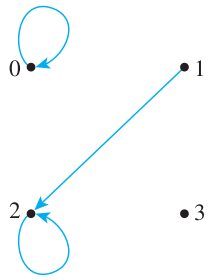
\includegraphics[scale=0.4]{../images/8.1.13.png}
\end{figure}
\end{proof}

\subsection{Exercise 14}
Define a relation $S$ on \(B = \{a, b, c, d\}\) by \(S = \{(a, b), (a, c), (b, c), (d, d)\}\).

\begin{proof}
\begin{figure}[ht!]
\centering
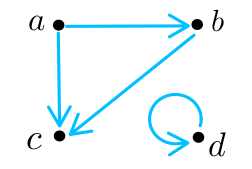
\includegraphics[scale=0.4]{../images/8.1.14.png}
\end{figure}
\end{proof}

\subsection{Exercise 15}
Let \(A = \{2, 3, 4, 5, 6, 7, 8\}\) and define a relation $R$ on $A$ as follows: For every \(x, y \in A, x \, R\, y 
\iff x \mid y\).

\begin{proof}
\begin{figure}[ht!]
\centering
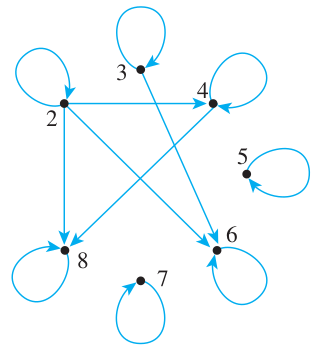
\includegraphics[scale=0.4]{../images/8.1.15.png}
\end{figure}
\end{proof}

\subsection{Exercise 16}
Let \(A = \{5, 6, 7, 8, 9, 10\}\) and define a relation $S$ on $A$ as follows: For every \(x, y \in A, x \, S \, y \iff 
2 \mid (x - y)\).

\begin{proof}
\begin{figure}[ht!]
\centering
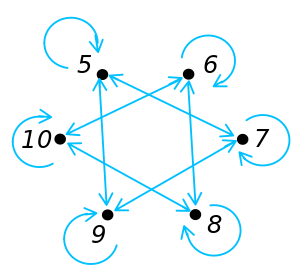
\includegraphics[scale=0.4]{../images/8.1.16.png}
\end{figure}
\end{proof}

\subsection{Exercise 17}
Let \(A = \{2, 3, 4, 5, 6, 7, 8\}\) and define a relation $T$ on $A$ as follows: For every \(x, y \in A, x \, T \, y 
\iff 3 \mid (x - y)\).

\begin{proof}
\begin{figure}[ht!]
\centering
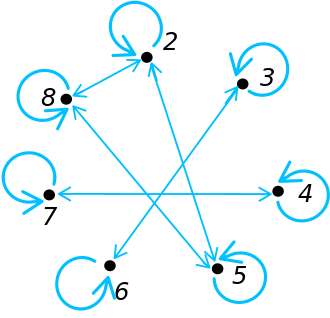
\includegraphics[scale=0.4]{../images/8.1.17.png}
\end{figure}
\end{proof}

\subsection{Exercise 18}
Let \(A = \{0, 1, 3, 4, 5, 6\}\) and define a relation $V$ on $A$ as follows: For every \(x, y \in A, x \, V \, y \iff 
5 \mid (x^2 - y^2)\).

\begin{proof}
\begin{figure}[ht!]
\centering
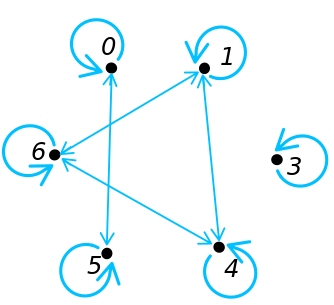
\includegraphics[scale=0.4]{../images/8.1.18.png}
\end{figure}
\end{proof}

\subsection{Exercise 19}
Let \(A = \{2, 4\}\) and \(B = \{6, 8, 10\}\) and define relations $R$ and $S$ from $A$ to $B$ as follows: For every 
\((x, y) \in A \times B, x \, R \, y \iff x \mid y\) and \( x \, S \, y \iff y - 4 = x\). State explicitly which 
ordered pairs are in \(A \times B, R, S, R \cup S\), and \(R \cap S\).

\begin{proof}
\(A \times B = \{(2, 6), (2, 8), (2, 10), (4, 6), (4, 8), (4, 10)\}\)

\(R = \{(2, 6), (2, 8), (2, 10), (4, 8)\}\), \(S = \{(2, 6), (4, 8)\}\), \(R \cup S = R, R \cap S = S\)
\end{proof}

\subsection{Exercise 20}
Let \(A = \{-1, 1, 2, 4\}\) and \(B = \{1, 2\}\) and define relations $R$ and $S$ from $A$ to $B$ as follows: For every 
\((x, y) \in A \times B, x \, R \, y \iff |x| \mid |y|\) and \(x \, S \, y \iff x - y\) is even. State explicitly 
which ordered pairs are in \(A \times B, R, S, R \cup S\), and \(R \cap S\).

\begin{proof}
\(A \times B = \{(-1, 1), (-1, 2), (1, 1), (1, 2), (2, 1), (2, 2), (4, 1), (4, 2)\}\)

\(R = \{(-1, 1), (1, 1), (2, 2)\}\), \(S = \{(-1, 1), (1, 1), (2, 2), (4, 2)\}\), \(R \cup S = S, R \cap S = R\)
\end{proof}

\subsection{Exercise 21}
Define relations $R$ and $S$ on $R$ as follows: \(R = \{(x, y) \in \R \times \R \, | \, x < y\}\) and 

\(S = \{(x, y) \in \R \times \R \, | \, x = y\}\). That is, $R$ is the “less than” relation and $S$ is the “equals” 
relation on $\R$. Graph \(R, S, R \cup S\), and \(R \cap S\) in the Cartesian plane.

\begin{proof}
The graph of the intersection of $R$ and $S$ is obtained by finding the set of all points common to both graphs. But 
there are no points for which both \(x < y\) and \(x = y\). Hence \(R \cap S = \es\) and the graph consists of no 
points at all.

\begin{figure}[ht!]
\centering
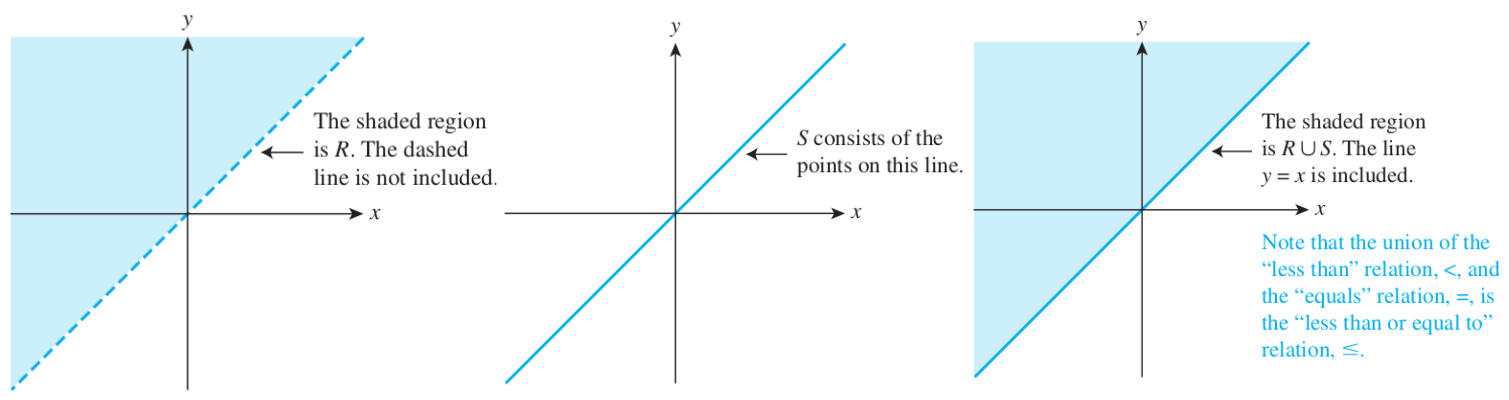
\includegraphics[scale=0.35]{../images/8.1.21.png}
\end{figure}
\end{proof}

\subsection{Exercise 22}
Define relations $R$ and $S$ on $R$ as follows: \(R = \{(x, y) \in \R \times \R \, | \, x^2 + y^2 = 4\}\) and 
\(S = \{(x, y) \in \R \times \R \, | \, x = y\}\). Graph \(R, S, R \cup S\), and \(R \cap S\) in the Cartesian plane.

\begin{proof}
\begin{figure}[ht!]
\centering
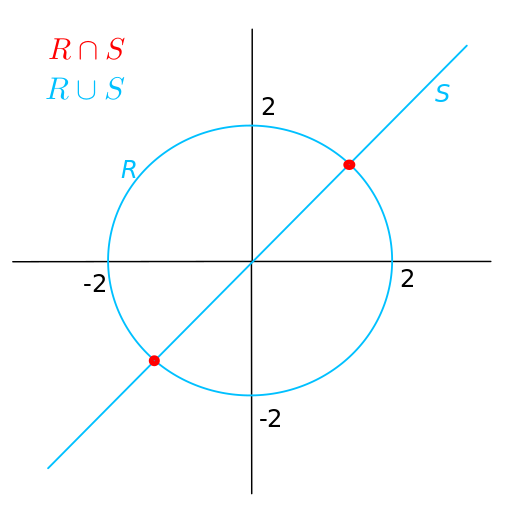
\includegraphics[scale=0.3]{../images/8.1.22.png}
\end{figure}
\end{proof}

\subsection{Exercise 23}
Define relations $R$ and $S$ on $R$ as follows: \(R = \{(x, y) \in \R \times \R \, | \, y = |x|\}\) and 
\(S = \{(x, y) \in \R \times \R \, | \, y = 1\}\). Graph \(R, S, R \cup S\), and \(R \cap S\) in the Cartesian plane.

\begin{proof}
\begin{figure}[ht!]
\centering
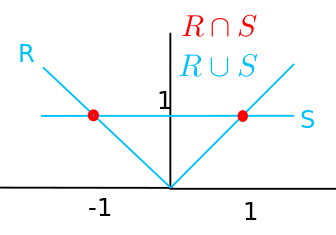
\includegraphics[scale=0.35]{../images/8.1.23.png}
\end{figure}
\end{proof}

\subsection{Exercise 24}
In Example 8.1.7 consider the query SELECT Patient\_ID\#, Name FROM S WHERE Primary\_Diagnosis = $X$. The response to 
the query is the projection onto the first two coordinates of the intersection of the database with the set 
\(A_1 \times A_2 \times A_3 \times \{X\}\).

\subsubsection{(a)}
Find the result of the query SELECT Patient\_ID\#, Name FROM S WHERE Primary\_Diagnosis = pneumonia.

\begin{proof}
574329 Tak Kurosawa, 011985 John Schmidt
\end{proof}

\subsubsection{(b)}
Find the result of the query SELECT Patient\_ID\#, Name FROM S WHERE Primary\_Diagnosis = appendicitis.

\begin{proof}
466581 Mary Lazars, 778400 Jamal Baskers
\end{proof}

\section{Exercise Set 8.2}

{\bf \cy In $1-8$, a number of relations are defined on the set \(A = \{0, 1, 2, 3\}\). For each relation:

a. Draw the directed graph.

b. Determine whether the relation is reflexive.

c. Determine whether the relation is symmetric.

d. Determine whether the relation is transitive.

Give a counterexample in each case in which the relation does not satisfy one of the properties.}

\subsection{Exercise 1}
\(R_1 = \{(0, 0), (0, 1), (0, 3), (1, 1), (1, 0), (2, 3), (3, 3)\}\)

\subsubsection{(a)}

\begin{proof}
\begin{figure}[ht!]
\centering
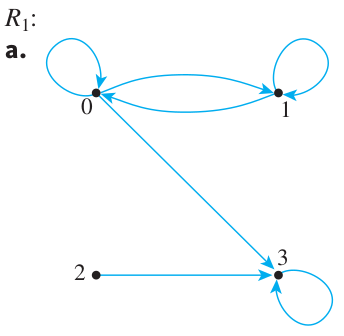
\includegraphics[scale=0.35]{../images/8.2.1.a.png}
\end{figure}
\end{proof}

\subsubsection{(b)}
\begin{proof}
$R_1$ is not reflexive: \(2 \,\Ccancel{R_1} \, 2\).
\end{proof}

\subsubsection{(c)}
\begin{proof}
$R_1$ is not symmetric: \(2 \,R_1\, 3\) but \(3 \, \Ccancel{R_1} \,2\).
\end{proof}

\subsubsection{(d)}
\begin{proof}
$R_1$ is not transitive: \(1 \,R_1\, 0\) and \(0 \,R_1\, 3\) but \(1 \,\Ccancel{R_1}\, 3\).
\end{proof}

\subsection{Exercise 2}
\(R_2 = \{(0, 0), (0, 1), (1, 1), (1, 2), (2, 2), (2, 3)\}\)

\subsubsection{(a)}
\begin{proof}
\begin{figure}[ht!]
\centering
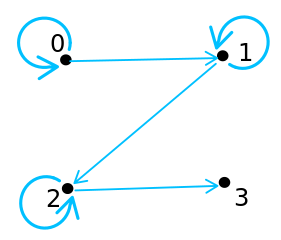
\includegraphics[scale=0.35]{../images/8.2.2.a.png}
\end{figure}
\end{proof}

\subsubsection{(b)}
\begin{proof}
$R_2$ is not reflexive: \(3 \, \Ccancel{R_2} \,3\).
\end{proof}

\subsubsection{(c)}
\begin{proof}
$R_2$ is not symmetric: \(2 \,R_2 \,3\) but \(3\, \Ccancel{R_2} \,2\).
\end{proof}

\subsubsection{(d)}
\begin{proof}
$R_2$ is not transitive: \(0\, R_2\, 1\) and \(1 \,R_2 \,2\) but \(0 \,\Ccancel{R_2}\, 2\).
\end{proof}

\subsection{Exercise 3}
\(R_3 = \{(2, 3), (3, 2)\}\)

\subsubsection{(a)}

\begin{proof}
\begin{figure}[ht!]
\centering
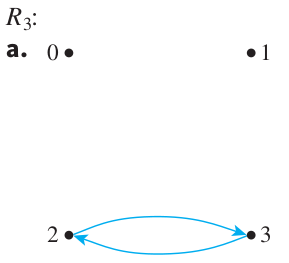
\includegraphics[scale=0.4]{../images/8.2.3.a.png}
\end{figure}
\end{proof}

\subsubsection{(b)}

\begin{proof}
$R_3$ is not reflexive: \(0 \, \Ccancel{R_3} \,0\).
\end{proof}

\subsubsection{(c)}

\begin{proof}
$R_3$ is symmetric.
\end{proof}

\subsubsection{(d)}

\begin{proof}
$R_3$ is not transitive: \(2\, R_3\, 3\) and \(3 \,R_3 \,2\) but \(2 \,\Ccancel{R_3}\, 2\).
\end{proof}

\subsection{Exercise 4}
\(R_4 = \{(1, 2), (2, 1), (1, 3), (3, 1)\}\)

\subsubsection{(a)}

\begin{proof}
\begin{figure}[ht!]
\centering
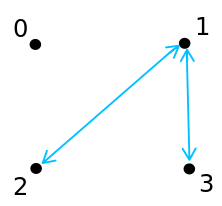
\includegraphics[scale=0.4]{../images/8.2.4.a.png}
\end{figure}
\end{proof}

\subsubsection{(b)}

\begin{proof}
$R_4$ is not reflexive: \(0 \, \Ccancel{R_4} \,0\).
\end{proof}

\subsubsection{(c)}

\begin{proof}
$R_4$ is symmetric.
\end{proof}

\subsubsection{(d)}

\begin{proof}
$R_4$ is not transitive: \(2\, R_4\, 1\) and \(1 \,R_4 \,3\) but \(2 \,\Ccancel{R_4}\, 3\).
\end{proof}

\subsection{Exercise 5}
\(R_5 = \{(0, 0), (0, 1), (0, 2), (1, 2)\}\)

\subsubsection{(a)}

\begin{proof}
\begin{figure}[ht!]
\centering
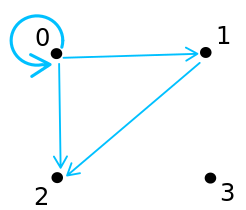
\includegraphics[scale=0.35]{../images/8.2.5.a.png}
\end{figure}
\end{proof}

\subsubsection{(b)}

\begin{proof}
$R_5$ is not reflexive: \(3 \, \Ccancel{R_5} \, 3\).
\end{proof}

\subsubsection{(c)}

\begin{proof}
$R_5$ is not symmetric: \(1 \,R_5 \,2\) but \(2\, \Ccancel{R_5} \,1\).
\end{proof}

\subsubsection{(d)}

\begin{proof}
$R_5$ is transitive.
\end{proof}

\subsection{Exercise 6}
\(R_6 = \{(0, 1), (0, 2)\}\)

\subsubsection{(a)}

\begin{proof}
\begin{figure}[ht!]
\centering
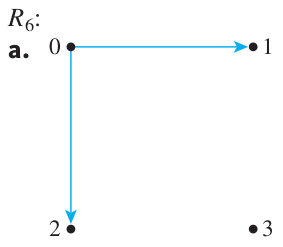
\includegraphics[scale=0.35]{../images/8.2.6.a.png}
\end{figure}
\end{proof}

\subsubsection{(b)}

\begin{proof}
$R_6$ is not reflexive: \(3 \, \Ccancel{R_6} \, 3\).
\end{proof}

\subsubsection{(c)}

\begin{proof}
$R_6$ is not symmetric: \(0 \,R_6 \,1\) but \(1\, \Ccancel{R_6} \,0\).
\end{proof}

\subsubsection{(d)}

\begin{proof}
$R_6$ is transitive.
\end{proof}

\subsection{Exercise 7}
\(R_7 = \{(0, 3), (2, 3)\}\)

\subsubsection{(a)}

\begin{proof}
\begin{figure}[ht!]
\centering
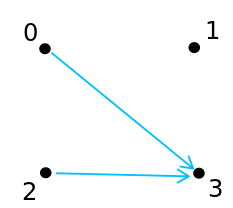
\includegraphics[scale=0.35]{../images/8.2.7.a.png}
\end{figure}
\end{proof}

\subsubsection{(b)}

\begin{proof}
$R_7$ is not reflexive: \(3 \, \Ccancel{R_7} \, 3\).
\end{proof}

\subsubsection{(c)}

\begin{proof}
$R_7$ is not symmetric: \(0 \,R_7 \, 3\) but \(3\, \Ccancel{R_7} \,0\).
\end{proof}

\subsubsection{(d)}

\begin{proof}
$R_7$ is transitive.
\end{proof}

\subsection{Exercise 8}
\(R_8 = \{(0, 0), (1, 1)\}\)

\subsubsection{(a)}

\begin{proof}
\begin{figure}[ht!]
\centering
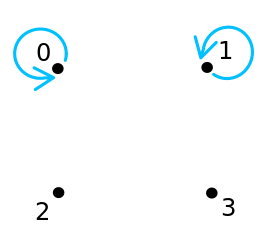
\includegraphics[scale=0.35]{../images/8.2.8.a.png}
\end{figure}
\end{proof}

\subsubsection{(b)}

\begin{proof}
$R_8$ is not reflexive: \(3 \, \Ccancel{R_8} \, 3\).
\end{proof}

\subsubsection{(c)}

\begin{proof}
$R_8$ is symmetric.
\end{proof}

\subsubsection{(d)}

\begin{proof}
$R_8$ is transitive.
\end{proof}

{\bf \cy In 9–33, determine whether the given relation is reflexive, symmetric, transitive, or none of these. 
Justify your answers. }

\subsection{Exercise 9}
$R$ is the “greater than or equal to” relation on the set of real numbers: For every \(x, y \in \R, x \, R \, y \iff 
x \geq y\).

\begin{proof}
{\bf \(\bm{R}\) is reflexive:} \(R\) is reflexive iff for every real number \(x, x \, R \, x\). By definition of 
\(R\), this means that for every real number \(x, x \geq x\). In other words, for every real number \(x, x > x\) or 
\(x = x\), which is true.

{\bf \(\bm{R}\) is not symmetric:} \(R\) is symmetric iff for all real numbers \(x\) and \(y\), if \(x \, R \, y\) 
then \(y \, R \, x\). By definition of \(R\), this means that for all real numbers \(x\) and \(y\), if \(x \geq y\) 
then \(y \geq x\). The following counterexample shows that this is false. \(x = 1\) and \(y = 0\). Then \(x \geq y\), 
but \(y \ngeq x\) because \(1 \geq 0\) and \(0 \ngeq 1\).

{\bf \(\bm{R}\) is transitive:} \(R\) is transitive iff for all real numbers \(x, y\), and \(z\), if \(x \, R \, y\) 
and \(y \, R \, z\) then \(x \, R \, z\). By definition of \(R\), this means that for all real numbers \(x, y\), and 
\(z\), if \(x \geq y\) and \(y \geq z\) then \(x \geq z\). This is true by definition of \(\geq\) and the transitive 
property of order for the real numbers. (See Appendix A, T18.)
\end{proof}

\subsection{Exercise 10}
$C$ is the circle relation on the set of real numbers: For every \(x, y \in \R, x \, C \, y \iff x^2 + y^2 = 1\).

\begin{proof}
{\bf \(\bm{C}\) is not reflexive:} Let \(x = 0\). Then \(0^2 + 0^2 = 0 \neq 1\), therefore \(0 \Ccancel{C} 0\).

{\bf \(\bm{C}\) is symmetric:} Assume \(x \, C \, y\). Then \(x^2 + y^2 = 1\). So \(y^2 + x^2 = 1\). So \(y\, C \, x\).

{\bf \(\bm{C}\) is not transitive:} Let \(x = 1, y = 0, z = 1\). Then \(x \, C \, y\) because \(1^2 + 0^2 = 1\), and
\(y \, C \, z\) because \(0^2 + 1^2 = 1\). However \(x \, \Ccancel{C} \, z\) because \(1^2 + 1^2 = 2 \neq 1\).
\end{proof}

\subsection{Exercise 11}
$D$ is the relation defined on $\R$ as follows: For every \(x, y \in \R, x \, D \, y \iff xy \geq 0\).

\begin{proof}
{\bf \(\bm{D}\) is reflexive:} For all real numbers \(x, x \cdot x = x^2 \geq 0\) so \(x \, D \, x\).

{\bf \(\bm{D}\) is symmetric:} Assume \(x \, D \, y\). Then \(xy \geq 0\). So \(yx \geq 0\). So \(y \, D \, x\). 

{\bf \(\bm{D}\) is not transitive:} Let \(x = 1, y = 0, z = -1\). Then \(xy = 0 \geq 0\) so \(x \, D \, y\), and
\(yz = 0 \geq 0\) so \(y \, D \, z\), but \(xz = -1 \ngeq 0\) so \(x \Ccancel{D} z\).
\end{proof}

\subsection{Exercise 12}
$E$ is the congruence modulo 4 relation on $\Z$: For every \(m, n \in \Z, m \, E \, n \iff 4 \mid (m - n)\).

\begin{proof}
{\bf \(\bm{E}\) is reflexive:} For all \(m \in \Z, (m-m) = 0 = 4 \cdot 0\) so \(4 \mid (m-m)\) thus \(m\,E\,m\).

{\bf \(\bm{E}\) is symmetric:} Assume \(m \, E \, n\). Then \(4\mid(m-n)\). So \(m-n = 4\cdot k\) for some integer $k$.
So \(n-m = 4 \cdot (-k)\) where $-k$ is an integer. So \(4 \mid (n-m)\) and \(n \, E \, m\).

{\bf \(\bm{E}\) is transitive:} Assume \(m \, E \, n\) and \(n \, E \, o\). Then \(4 \mid (m-n)\) and \(4\mid (n-o)\).
So \(m-n = 4k\) and \(n-o = 4l\) for some integers \(k,l\). So \(m-o = (m-n) + (n-o) = 4k+4l = 4(k+l)\) where \(k+l\) 
is an integer. Thus \(4 \mid (m-o)\) and \(m \,E\,o\).
\end{proof}

\subsection{Exercise 13}
$F$ is the congruence modulo 5 relation on $\Z$: For every \(m, n \in \Z, m \, F \, n \iff 5 \mid (m - n)\).

\begin{proof}
{\bf \(\bm{F}\) is reflexive:} The proof is the same as in exercise 12.

{\bf \(\bm{F}\) is symmetric:} The proof is the same as in exercise 12.

{\bf \(\bm{F}\) is transitive:} The proof is the same as in exercise 12.
\end{proof}

\subsection{Exercise 14}
$O$ is the relation defined on $\Z$ as follows: For every \(m, n \in \Z, m \, O \, n \iff m - n\) is odd.

\begin{proof}
{\bf \(\bm{O}\) is not reflexive:} \(0 - 0 = 0\) is even, therefore \(0 \Ccancel{O} 0\).

{\bf \(\bm{O}\) is symmetric:} Assume \(m \, O \, n\). So \(m-n\) is odd. So \(m-n = 2k+1\) for some integer \(k\). So
\(n-m = -2k-1 = 2(-k-1)+1\) where \(-k-1\) is an integer. So \(n-m\) is odd and \(n \, O \, m\).

{\bf \(\bm{O}\) is not transitive:} \(2 - 1 = 1\) is odd so \(2 \, O \, 1\), and \(1 - 0 = 1\) is odd so \(1 \,O\,0\),
but \(2-0 = 2\) is even so \(2 \Ccancel{O} 0\).
\end{proof}

\subsection{Exercise 15}
$D$ is the “divides” relation on \(Z^+\): For all positive integers $m$ and \(n, m \, D \, n \iff m \mid n\).

\begin{proof}
{\bf \(\bm{D}\) is reflexive:} For all \(m \in \Z^+\) \(m = m \cdot 1\) therefore \(m \mid m\), so \(m \, D \, m\).

{\bf \(\bm{D}\) is not symmetric:} \(3 \, D \, 6\) because \(3 \mid 6\) because \(6 = 3 \cdot 2\), but \(6 \Ccancel{D}
3\) because \(6 \nmid 3\) since \(3 / 6 = 1/2\) is not an integer.

{\bf \(\bm{D}\) is transitive:} Assume \(m \, D \, n\) and \(n \, D \, o\). Then \(m \mid n\) and \(n \mid o\). So
\(n = mk\) and \(o = nl\) for some integers \(k, l\). So \(o = nl = (mk)l = m(kl)\) where \(kl\) is an integer. So
\(m \mid o\) and \(m \, D \, o\).
\end{proof}

\subsection{Exercise 16}
$A$ is the “absolute value” relation on $\R$: For all real numbers $x$ and $y$, \(x \, A \, y \iff |x| = |y|\).

\begin{proof}
{\bf \(\bm{A}\) is reflexive:} For all real numbers \(x, |x| = |x|\) so \(x \, A \, x\).

{\bf \(\bm{A}\) is symmetric:} Assume \(x \, A \, y\) so \(|x| = |y|\). Then \(|y| = |x|\) so \(y \, A \, x\).

{\bf \(\bm{A}\) is transitive:} Assume \(x \, A \, y\) and \(y \, A \, z\), so \(|x| = |y|\) and \(|y| = |z|\). Then
\(|x| = |y| = |z|\) so \(x \, A \, z\).
\end{proof}

\subsection{Exercise 17}
Recall that a prime number is an integer that is greater than 1 and has no positive integer divisors other than 1 
and itself. (In particular, 1 is not prime.) A relation $P$ is defined on $\Z$ as follows: For every \(m, n \in \Z, m 
\, P \, n \iff \exists\) a prime number $p$ such that \(p \mid m\) and \(p \mid n\).

\begin{proof}
{\bf \(\bm{P}\) is not reflexive:} There is no prime number $p$ such that \(p \mid 1\) and \(p \mid 1\). Thus
\(1 \Ccancel{P} 1\).

{\bf \(\bm{P}\) is symmetric:} Assume \(m \, P \, n\). So there is a prime number $p$ such that \(p \mid m\) and 
\(p \mid n\). So \(p \mid n\) and \(p \mid m\), and thus \(n \, P \, m\).

{\bf \(\bm{P}\) is not transitive:} Let \(m = 6, n = 15, o = 35\). Then the prime $p = 3$ divides both $m$ and $n$, so
\(m \, P \, n\), and the prime $q = 5$ divides both $n$ and $o$, so \(n \, P \, o\), but there is no prime that divides
both $m = 2 \cdot 3$ and $o = 5 \cdot 7$, so \(m \Ccancel{P} o\).
\end{proof}

\subsection{Exercise 18}
Define a relation $Q$ on $\R$ as follows: For all real numbers $x$ and $y$, \(x \, Q \, y \iff x - y\) is 
rational.

\begin{proof}
{\bf \(\bm{Q}\) is reflexive:} For all reals \(x \in \R, x-x = 0\) and 0 is rational, so \(x \, Q \, x\).

{\bf \(\bm{Q}\) is symmetric:} Assume \(x \, Q \, y\). Then \(x - y\) is rational. Then \(y-x = -(x-y)\) is rational 
(being the negative of a rational). So \(y \, Q \, x\).

{\bf \(\bm{Q}\) is transitive:} Assume \(x \, Q \, y\) and \(y \, Q \, z\). Then \(x - y\) and \(y - z\) are rational.
So \(x - z = (x-y) + (y-z)\) is also rational (being the sum of two rationals). Thus \(x \, Q \, z\).
\end{proof}

\subsection{Exercise 19}
Define a relation $I$ on $\R$ as follows: For all real numbers $x$ and $y$, \(x \, I \, y \iff x - y\) is 
irrational.

\begin{proof}
{\bf \(\bm{I}\) is not reflexive:} For all reals \(x \in \R, x - x = 0\) and 0 is not irrational, 
so \(x \Ccancel{I} x\).

{\bf \(\bm{I}\) is symmetric:} Assume \(x \, I \, y\). Then \(x - y\) is irrational. So \(y-x = -(x-y)\) is irrational 
(being the negative of an irrational). So \(y \, I \, x\).

{\bf \(\bm{I}\) is not transitive:} Let \(x = \sqrt{2}, y = 0, z = \sqrt{2}\). Then \(x \, I \, y\) because \(x - y = 
\sqrt{2}\) is irrational. Also \(y \, I \, z\) because \(y - z = -\sqrt{2}\) is irrational. But \(x - z = 0\) is not
irrational, thus \(x \Ccancel{I} z\).
\end{proof}

\subsection{Exercise 20}
Let \(X = \{a, b, c\}\) and \(\ps(X)\) be the power set of $X$ (the set of all subsets of $X$). A relation {\bf E} is 
defined on \(\ps(X)\) as follows: For every \(A, B \in \ps(X), A \,\textbf{E}\, B \iff \) the number of elements 
in $A$ equals the number of elements in $B$.

\begin{proof}
{\bf E is reflexive:} For every \(A \in \ps(X)\), the number of elements in $A$ equals the number of elements in 
$A$. So \(A \,\textbf{E}\, A\).

{\bf E is symmetric:} Assume \(A \,\textbf{E}\, B\). Then the number of elements in $A$ equals the number of elements 
in $B$. So, the number of elements in $B$ equals the number of elements in $A$. So \(B \,\textbf{E}\, A\).

{\bf E is transitive:} Assume \(A \,\textbf{E}\, B\) and \(B \,\textbf{E}\, C\). Then the number of elements in $A$ 
equals the number of elements in $B$, and the number of elements in $B$ equals the number of elements in $C$. So 
the number of elements in $A$ equals the number of elements 
in $C$. So \(A \,\textbf{E}\, C\).
\end{proof}

\subsection{Exercise 21}
Let \(X = \{a, b, c\}\) and \(\ps(X)\) be the power set of $X$. A relation {\bf L} is defined on \(\ps(X)\) as 
follows: For every \(A, B \in \ps(X), A \,\textbf{L}\, B \iff \) the number of elements in $A$ is less than the 
number of elements in $B$.

\begin{proof}
{\bf L is not reflexive:} For all \(A \in \ps(X)\), the number of elements in $A$ is not less than the number of 
elements in $A$. So \(A \,\Ccancel{\textbf{L}}\, A\).

{\bf L is not symmetric:} Let \(A = \es, B = \{a\}\). Then the number of elements in $A$ (which is 0) is less than the 
number of elements in $B$ (which is 1). So \(A \,\textbf{L}\, B\). But the number of elements in $B$ (which is 1) is 
not less than the number of elements in $A$ (which is 0). So \(B\,\Ccancel{\textbf{L}}\, A\).

{\bf L is transitive:} Assume \(A \, \textbf{L} \, B\) and \(B \, \textbf{L} \, C\). Then the number of elements in 
$A$ is less than the number of elements in $B$, and the number of elements in $B$ is less than the number of 
elements in $C$. Then the number of elements in $A$ is less than the number of elements in $C$. So \(A \, \textbf{L} \, C\).
\end{proof}

\subsection{Exercise 22}
Let \(X = \{a, b, c\}\) and \(\ps(X)\) be the power set of $X$. A relation {\bf N} is defined on \(\ps(X)\) as 
follows: For every \(A, B \in \ps(X), A \textbf{N} B \iff \) the number of elements in $A$ is not equal to the number 
of elements in $B$.

\begin{proof}
{\bf N is not reflexive:} Let \(A = \{a\}\) which has 1 element. Then the number of elements in $A$ is equal to the number of elements in $A$. So \(A \,\Ccancel{\textbf{N}}\, A\).

{\bf N is symmetric:} Assume \(A \,\textbf{N}\, B\). Then the number of elements in $A$ is not equal to the number 
of elements in $B$. So the number of elements in $B$ is not equal to the number of elements in $A$, and 
\(B \,\textbf{N}\, A\).

{\bf N is not transitive:} Let \(A = \{a\}, B = \es, C = \{c\}\). Then \(A \,\textbf{N}\, B\) because $A$ has 1 
element and $B$ has 0 elements, and $0 \neq 1$. Similarly \(B \,\textbf{N}\, C\). But \(A \,\Ccancel{\textbf{N}}\, C\)
because both $A$ and $C$ have 1 element, and 1 = 1.
\end{proof}

\subsection{Exercise 23}
Let $X$ be a nonempty set and \(\ps(X)\) the power set of $X$. Define the “subset” relation {\bf S} on \(\ps(X)\) as 
follows: For every \(A, B \in \ps(X), A \,\textbf{S}\, B \iff A \subseteq B\).

\begin{proof}
{\bf S is reflexive:} For all \(A \in \ps(X), A \subseteq A\) therefore \(A \,\textbf{S}\, A\).

{\bf S is not symmetric:} Let \(A = \{a\}, B = \{a, b\}\). Then \(A \subseteq B\), so \(A \,\textbf{S}\, B\). But 
\(B \nsubseteq A\) therefore \(B \,\Ccancel{\textbf{S}}\, A\).

{\bf S is transitive:} Assume \(A \,\textbf{S}\, B\) and \(B \,\textbf{S}\, C\). So \(A \subseteq B\) and 
\(B \subseteq C\). Then by transitivity of subsets, \(A \subseteq C\), and \(A \,\textbf{S}\, C\).
\end{proof}

\subsection{Exercise 24}
Let \(X\) be a nonempty set and \(\ps(X)\) the power set of $X$. Define the “not equal to” relation {\bf U} on 
\(\ps(X)\) as follows: For every \(A, B \in \ps(X), A \textbf{U} B \iff A \neq B\).

\begin{proof}
{\bf U is not reflexive:} For every \(A \in \ps(X), A = A\) therefore \(A \, \Ccancel{\textbf{U}} \, A\).

{\bf U is symmetric:} Assume \(A \, \textbf{U} \, B\). Then \(A \neq B\). So \(B \neq A\), and \(B \,\textbf{U} \, A\).

{\bf U is not transitive:} Let \(X = \{x\}, A = \{x\}, B = \es, C = \{x\}\). Then \(A \, \textbf{U} \, B\) because 
\(A \neq B\), and \(B\,\textbf{U}\,C\) because \(B \neq C\), but \(A = C\) so \(A \, \Ccancel{\textbf{U}} \, C\).
\end{proof}

\subsection{Exercise 25}
Let $A$ be the set of all strings of $a$’s and $b$’s of length 4. Define a relation \(R\) on \(A\) as follows: For 
every \(s, t \in A, s \, R \, t \iff s\) has the same first two characters as \(t\).

\begin{proof}
{\bf \(\bm{R}\) is reflexive:} For every string \(s \in A\), $s$ has the same first two characters as $s$. Thus
\(s \, R \, s\).

{\bf \(\bm{R}\) is symmetric:} Assume \(s \, R \, t\). Then $s$ has the same first two characters as $t$. Then $t$ has
the same first two characters as $s$, so \(t \, R \, s\).

{\bf \(\bm{R}\) is transitive:} Assume \(s \, R \, t\) and \(t \, R \, r\). Then $s$ has the same first two characters 
as $t$, and $t$ has the same first two characters as $r$. So $s$ has the same first two characters as $r$, and 
\(s \, R \, r\).
\end{proof}

\subsection{Exercise 26}
Let \(A\) be the set of all strings of 0’s, 1’s, and 2’s that have length 4 and for which the sum of the characters 
in the string is less than or equal to 2. Define a relation \(R\) on \(A\) as follows: For every \(s, t \in A, s \, R 
\, t \iff\) the sum of the characters of \(s\) equals the sum of the characters of \(t\).

\begin{proof}
{\bf \(\bm{R}\) is reflexive:} For every \(s, \in A\), the sum of the characters of \(s\) equals the sum of the 
characters of \(s\). So \(s \, R \, s\).

{\bf \(\bm{R}\) is symmetric:} Assume \(s \, R \, t\). Then the sum of the characters of \(s\) equals the sum of the 
characters of \(t\). So the sum of the characters of \(t\) equals the sum of the characters of \(s\), and \(s\,R\,t\).

{\bf \(\bm{R}\) is transitive:} Assume \(s \, R \, t\) and \(t \, R \, r\). Then the sum of the characters of \(s\) 
equals the sum of the characters of \(t\), and the sum of the characters of \(t\) equals the sum of the characters of 
\(r\). So the sum of the characters of \(s\) equals the sum of the characters of \(r\), and \(s\,R\,r\).
\end{proof}

\subsection{Exercise 27}
Let \(A\) be the set of all English statements. A relation {\bf I} is defined on \(A\) as follows: For every \(p, q 
\in A, p \,\textbf{I}\, q \iff p \implies q\) is true.

\begin{proof}
{\bf I is reflexive:} For every \(p \in A, p \implies p\) is true, therefore \(p \, \textbf{I} \, p\).

{\bf I is not symmetric:} Let $p$ be ``$1 is greater than 2$'' and let $q$ be ``2 is greater than 1''. So $p$ is 
false and $q$ is true. Therefore \(p \implies q\) is true and \(q \implies p\) is false. So \(p \, \textbf{I} \, q\)
but \(q \, \Ccancel{\textbf{I}} \, p\).

{\bf I is transitive:} Assume \(p \, \textbf{I} \, q\) and \(q \, \textbf{I} \, r\). So \(p \implies q\) is true and
\(q \implies r\) is true. By transitivity of implication, \(p \implies r\) is true, and \(p \, \textbf{I} \, r\).
\end{proof}

\subsection{Exercise 28}
Let \(A = \R \times \R\). A relation {\bf F} is defined on \(A\) as follows: For every \((x_1, y_1)\) and \((x_2, y_2)
\) in $A$, \((x_1, y_1) \textbf{F} (x_2, y_2) \iff x_1 = x_2\).

\begin{proof}
{\bf F is reflexive:} For every \((x, y) \in A, x = x\), therefore \((x, y) \textbf{F} (x, y)\).

{\bf F is symmetric:} Assume \((x_1, y_1) \textbf{F} (x_2, y_2)\). Then \(x_1 = x_2\). Then \(x_2 = x_1\). So
\((x_2, y_2) \textbf{F} (x_1, y_1)\).

{\bf F is transitive:} Assume \((x_1, y_1) \textbf{F} (x_2, y_2)\) and \((x_2, y_2) \textbf{F} (x_3, y_3)\). Then
\(x_1 = x_2\) and \(x_2 = x_3\). Thus \(x_1 = x_3\) and so \((x_1, y_1) \textbf{F} (x_3, y_3)\).
\end{proof}

\subsection{Exercise 29}
Let \(A = \R \times \R\). A relation {\bf S} is defined on \(A\) as follows: For every \((x_1, y_1)\) and \((x_2, y_2)
\) in \(A, (x_1, y_1) \textbf{S} (x_2, y_2) \iff y_1 = y_2\).

\begin{proof}
{\bf S is reflexive:}

{\bf S is symmetric:}

{\bf S is transitive:}
\end{proof}

\subsection{Exercise 30}
Let \(A\) be the “punctured plane”; that is, \(A\) is the set of all points in the Cartesian plane except the origin 
(0, 0). A relation \(R\) is defined on \(A\) as follows: For every \(p_1\) and \(p_2\) in \(A, p_1 \, R \, p_2 \iff 
p_1\) and \(p_2\) lie on the same half line emanating from the origin.

\begin{proof}
{\bf \(\bm{R}\) is reflexive:} For all \(p \in A, p\) and \(p\) lie on the same half line emanating from the origin.
So \(p \, R \, p\).

{\bf \(\bm{R}\) is symmetric:} Assume \(p_1 \, R \, p_2\). Then \(p_1\) and \(p_2\) lie on the same half line 
emanating from the origin. Then \(p_2\) and \(p_1\) lie on the same half line emanating from the origin. So
\(p_2 \, R \, p_1\).

{\bf \(\bm{R}\) is transitive:} First notice that for any \(p \in A\) there is exactly one half line emanating from 
the origin on which $p$ lies.

Assume \(p_1 \, R \, p_2\) and \(p_2 \, R \, p_3\). Then \(p_1\) and \(p_2\) lie on the same half line emanating from 
the origin, say $l_1$. And \(p_2\) and \(p_3\) lie on the same half line emanating from the origin, say $l_2$. Since 
$p_2$ lies on both $l_1$ and $l_2$, by the previous paragraph \(l_1 = l_2\). Then \(p_1\) and \(p_3\) lie on 
the same half line emanating from the origin. So \(p_1 \, R \, p_3\).
\end{proof}

\subsection{Exercise 31}
Let \(A\) be the set of people living in the world today. A relation \(R\) is defined on \(A\) as follows: For all 
people \(p\) and \(q\) in \(A, p \, R \, q \iff p\) lives within 100 miles of \(q\).

\begin{proof}
{\bf \(\bm{R}\) is reflexive:} For every person $p$, $p$ lives within 0 miles of $p$, so in particular $p$ lives 
within 100 miles of $p$. Therefore \(p \, R \, p\).

{\bf \(\bm{R}\) is symmetric:} Assume \(p \, R \, q\). So $p$ lives within 100 miles of $q$. Then $q$ lives within 
100 miles of $p$. Thus \(q \, R \, p\).

{\bf \(\bm{R}\) is not transitive:} As a counterexample, take $p$ to be an inhabitant of Chicago, Illinois, $q$ an 
inhabitant of Kankakee, Illinois, and $r$ an inhabitant of Champaign, Illinois. Then \(p \,R\, q\) because Chicago is 
less than 100 miles from Kankakee, and \(q \,R\, r\) because Kankakee is less than 100 miles from Champaign, but 
\(p \, \Ccancel{R}\, r\) because Chicago is not less than 100 miles from Champaign.
\end{proof}

\subsection{Exercise 32}
Let \(A\) be the set of all lines in the plane. A relation \(R\) is defined on \(A\) as follows: For every \(l_1\) and 
\(l_2\) in \(A, l_1 \, R \, l_2 \iff l_1\) is parallel to \(l_2\). (Assume that a line is parallel to itself.)

\begin{proof}
{\bf \(\bm{R}\) is reflexive:} For every line \(l \in A, l\) is parallel to itself, therefore \(l \, R \, l\).

{\bf \(\bm{R}\) is symmetric:} Assume \(l_1 \, R \, l_2\). Then \(l_1\) is parallel to \(l_2\). Then \(l_2\) is 
parallel to \(l_1\), so \(l_2 \, R \, l_1\).

{\bf \(\bm{R}\) is transitive:} Assume \(l_1 \, R \, l_2\) and \(l_2 \, R \, l_3\). Then \(l_1\) is parallel to $l_2$
and \(l_2\) is parallel to $l_3$. By transitivity of parallelism \(l_1\) is parallel to \(l_3\) so \(l_1 \, R \, l_3\).
\end{proof}

\subsection{Exercise 33}
Let \(A\) be the set of all lines in the plane. A relation \(R\) is defined on \(A\) as follows: For every \(l_1\) and 
\(l_2\) in \(A, l_1 \, R \, l_2 \iff l_1\) is perpendicular to \(l_2\).

\begin{proof}
{\bf \(\bm{R}\) is not reflexive:} For evert line $l$ in $A$, $l$ is not perpendicular to itself ($l$ is parallel to
itself). Therefore \(l \,\Ccancel{R}\, l\).

{\bf \(\bm{R}\) is symmetric:} Assume \(l_1 \, R \, l_2\). Then \(l_1\) is perpendicular to \(l_2\). Then \(l_2\) is 
perpendicular to \(l_1\). So \(l_2 \, R \, l_1\).

{\bf \(\bm{R}\) is not transitive:} Let $l_1$ be the line $y = 0$, let $l_2$ be the line $x = 0$ and $l_3$ be the 
line $y = 1$. Then $l_2$ is perpendicular to both $l_1$ and $l_3$ so \(l_1 \, R \, l_2\) and \(l_2 \, R \, l_3\). But
$l_1$ is parallel to $l_3$ so \(l_1 \, \Ccancel{R} \,l_3\).
\end{proof}

{\bf \cy In $34-36$, assume that $R$ is a relation on a set $A$. Prove or disprove each statement.}

\subsection{Exercise 34}
If \(R\) is reflexive, then \(R^{-1}\) is reflexive.

\begin{proof}
Suppose $R$ is any reflexive relation on a set $A$. {\it [We must show that \(R^{-1}\) is reflexive. To show this, 
we must show that for every \(x\) in \(A, x \, R^{-1} x\).]} Given any element \(x\) in \(A\), since \(R\) is 
reflexive, \(x \,R\, x\), and by definition of relation, this means that \((x, x) \in R\). It follows, by definition 
of the inverse of a relation, that \((x, x) \in R^{-1}\), and so, by definition of relation, \(x \,R^{-1}\, x\) {\it 
[as was to be shown].}
\end{proof}

\subsection{Exercise 35}
If \(R\) is symmetric, then \(R^{-1}\) is symmetric.

\begin{proof}
Assume \(R\) is symmetric. {\it [We want to show \(R^{-1}\) is symmetric.]} Assume \(x \, R^{-1} \, y\). We need to 
show \(y \, R^{-1} \, x\). By definition of \(R^{-1}, y \, R \, x\). Since \(R\) is symmetric, \(x \, R \, y\). By
definition of \(R^{-1}\) again, \(y \, R^{-1} \, x\).
\end{proof}

\subsection{Exercise 36}
If \(R\) is transitive, then \(R^{-1}\) is transitive.

\begin{proof}
Assume \(R\) is transitive. {\it [We want to show \(R^{-1}\) is transitive.]} Assume \(x \, R^{-1} \, y\) and \(y \, 
R^{-1} \, z\). We need to show \(x \, R^{-1} \, z\). By definition of \(R^{-1}, y \, R \, x\) and \(z \, R \, y\). 
Since \(R\) is transitive, \(z \, R \, x\). By definition of \(R^{-1}\) again, \(x \, R^{-1} \, z\).
\end{proof}

{\bf \cy In $37-42$, assume that \(R\) and \(S\) are relations on a set \(A\). Prove or disprove each 
statement.}

\subsection{Exercise 37}
If \(R\) and \(S\) are reflexive, is \(R \cap S\) reflexive? Why?

\begin{proof}
Yes. Suppose $R$ and $S$ are reflexive. {\it [To show that \(R \cap S\) is reflexive, we must show that \(\forall x 
\in A, (x, x) \in R \cap S\).]} So suppose \(x \in A\). Since $R$ is reflexive, \((x, x) \in R\), and since $S$ is 
reflexive, \((x, x) \in S\). Thus, by definition of intersection, \((x, x) \in R \cap S\) {\it [as was to be shown].}
\end{proof}

\subsection{Exercise 38}
If \(R\) and \(S\) are symmetric, is \(R \cap S\) symmetric? Why?

\begin{proof}
Yes. Suppose $R$ and $S$ are symmetric. {\it [To show that \(R \cap S\) is symmetric, we must show that \(\forall x,y 
\in A\), if \((x, y) \in R \cap S\) then \((y, x) \in R \cap S\).]} So suppose \(x,y \in A\) and \((x, y) \in R 
\cap S\). By definition of intersection \((x, y) \in R\) and \((x,y)\in S\). Since $R$ is symmetric, \((y,x)\in R\), 
and since $S$ is symmetric, \((y, x) \in S\). Thus, by definition of intersection, \((y, x) \in R \cap S\) 
{\it [as was to be shown].}
\end{proof}

\subsection{Exercise 39}
If \(R\) and \(S\) are transitive, is \(R \cap S\) transitive? Why?

\begin{proof}
Yes. Suppose $R$ and $S$ are transitive. {\it [To show that \(R \cap S\) is transitive, we must show that \(\forall x,y 
,z \in A\), if \((x, y) \in R \cap S\) and \((y, z) \in R \cap S\) then \((x, z) \in R \cap S\).]} So suppose \(x,y,z 
\in A\) and \((x, y) \in R \cap S\) and \((y, z) \in R \cap S\). By definition of intersection \((x, y) \in R\) and 
\((x,y)\in S\) and \((y, z) \in R\) and \((y,z)\in S\). Since $R$ is transitive, \((x,z)\in R\), and since $S$ is 
transitive, \((x, z) \in S\). Thus, by definition of intersection, \((x, z) \in R \cap S\) {\it [as was to be shown].}
\end{proof}

\subsection{Exercise 40}
If \(R\) and \(S\) are reflexive, is \(R \cup S\) reflexive? Why?

\begin{proof}
Yes. To prove this we must show that for all $x$ in $A$, \((x, x) \in R \cup S\). So suppose \(x\) is a particular 
but arbitrarily chosen element in \(A\). {\it [We must show that \((x, x) \in R \cup S\).]} Then \((x, x) \in R\) 
because $R$ is reflexive, and hence \((x, x) \in R \cup S\) by definition of union, {\it [as was to be shown]}.
\end{proof}

\subsection{Exercise 41}
If \(R\) and \(S\) are symmetric, is \(R \cup S\) symmetric? Why?

\begin{proof}
Yes. To prove this we must show that for all $x$ and $y$ in $A$, if \((x, y) \in R \cup S\) then \((y, x) \in R \cup 
S\). So suppose \((x, y)\) is a particular but arbitrarily chosen element in \(R \cup S\). {\it [We must show that 
\((y, x) \in R \cup S\).]} By definition of union, \((x, y) \in R\) or \((x, y) \in S\). In case \((x, y) \in R\), then 
\((y, x) \in R\) because $R$ is symmetric, and hence \((y, x) \in R \cup S\) by definition of union. In case \((x, y) 
\in S\) then \((y, x) \in S\) because $S$ is symmetric, and hence \((y, x) \in R \cup S\) by definition of union. Thus, 
in both cases, \((y, x) \in R \cup S\) {\it [as was to be shown]}.
\end{proof}

\subsection{Exercise 42}
If \(R\) and \(S\) are transitive, is \(R \cup S\) transitive? Why?

\begin{proof}
No. Let \(A = \{a,b,c,d\}, R = \{(a,b),(b,c),(a,c)\}, S = \{(c,a),(a,d),(c,d)\}\). Then $R$ and $S$ are transitive but
\(R \cup S\) is not: \((a,c) \in R \cup S\) and \((c,a) \in R \cup S\) but \((a,a) \notin R \cup S\).
\end{proof}

{\bf \cy In \(43-50\), the following definitions are used: a relation on a set \(A\) is defined to be irreflexive if, 
and only if, for every \(x \in A, x \, \Ccancel[cyan]{R} \, x\); asymmetric if, and only if, for every \(x, y \in A\) 
if \(x \, R \, y\) then \(y \Ccancel[cyan]{R} x\); intransitive if, and only if, for every \(x, y, z \in A\), 
if \(x R y\) and \(y R z\) then \(x \Ccancel[cyan]{R} z\). For each of the relations in the referenced exercise, 
determine whether the relation is irreflexive, asymmetric, intransitive, or none of these.}

\subsection{Exercise 43}
Exercise 1
\begin{proof}
\(R_1\) is not irreflexive because \((0, 0) \in R_1\). \(R_1\) is not asymmetric because \((0, 1) \in R_1\) and 
\((1, 0) \in R_1\). \(R_1\) is not intransitive because \((0, 1) \in R_1\) and \((1, 0) \in R_1\) and \((0, 0) \in R_1\).
\end{proof}

\subsection{Exercise 44}
Exercise 2
\begin{proof}
Recall \(R_2 = \{(0, 0), (0, 1), (1, 1), (1, 2), (2, 2), (2, 3)\}\).

\(R_2\) is not irreflexive because \((0, 0) \in R_2\).

\(R_2\) is not asymmetric because \((0, 0) \in R_2\) and \((0, 0) \in R_2\).

\(R_2\) is not intransitive because \((0, 0) \in R_2\) and \((0,1) \in R_2\) and \((0,1) \in R_2\).
\end{proof}

\subsection{Exercise 45}
Exercise 3
\begin{proof}
$R_3$ is irreflexive because no element of $A$ is related by $R_3$ to itself. $R_3$ is not asymmetric because 
\((2, 3) \in R_3\) and \((3, 2) \in R_3\). $R_3$ is intransitive. To see why, observe that $R_3$ consists only 
of \((2, 3)\) and \((3, 2)\). Now \((2, 3) \in R_3\) and \((3, 2) \in R_3\) but \((2, 2) \notin R_3\). Also 
\((3, 2) \in R_3\) and \((2, 3) \in R_3\) but \((3, 3) \notin R_3\).
\end{proof}

\subsection{Exercise 46}
Exercise 4
\begin{proof}
Recall \(R_4 = \{(1, 2), (2, 1), (1, 3), (3, 1)\}\).

\(R_4\) is irreflexive.

\(R_4\) is not asymmetric because \((1, 2) \in R_4\) and \((2, 1) \in R_4\).

\(R_4\) is intransitive.
\end{proof}

\subsection{Exercise 47}
Exercise 5
\begin{proof}
Recall \(R_5 = \{(0, 0), (0, 1), (0, 2), (1, 2)\}\).

\(R_5\) is not irreflexive because \((0,0) \in R_5\).

\(R_5\) is not asymmetric because \((0, 0) \in R_5\) and \((0, 0) \in R_5\).

\(R_5\) is not intransitive because \((0,1) \in R_5\) and \((1,2) \in R_5\) and \((0,2) \in R_5\).
\end{proof}

\subsection{Exercise 48}
Exercise 6
\begin{proof}
Recall \(R_6 = \{(0, 1), (0, 2)\}\). \(R_6\) is irreflexive because no element of \(A\) is related by \(R_6\) to 
itself. \(R_6\) is asymmetric because \(R_6\) consists only of \((0, 1)\) and \((0, 2)\) and neither \((1, 0)\) nor 
\((2, 0)\) is in \(R_6\). \(R_6\) is intransitive.
\end{proof}

\subsection{Exercise 49}
Exercise 7
\begin{proof}
Recall \(R_7 = \{(0, 3), (2, 3)\}\).

\(R_7\) is irreflexive, asymmetric and intransitive.
\end{proof}

\subsection{Exercise 50}
Exercise 8
\begin{proof}
Recall \(R_8 = \{(0, 0), (1, 1)\}\). \(R_8\) is not irreflexive because \((0,0) \in R_8\). \(R_8\) is not 
asymmetric because \((0,0) \in R_8\) and \((0,0) \in R_8\).
\(R_8\) is intransitive.
\end{proof}

{\bf \cy In \(51-53, R, S\), and \(T\) are relations defined on \(A = \{0, 1, 2, 3\}\).}

\subsection{Exercise 51}
Let \(R = \{(0, 1), (0, 2), (1, 1), (1, 3), (2, 2), (3, 0)\}\). Find \(R^t\), the transitive closure of \(R\).

\begin{proof}
\(R^t = R \cup \{(0, 0), (0, 3), (1, 0), (3, 1), (3, 2), (3, 3), (0, 2), (1, 2)\} = \) 

\(\{(0, 0), (0, 1), (0, 2), (0, 3), (1, 0), (1, 1), (1, 2), (1, 3), (2, 2), (3, 0), (3, 1), (3, 2), (3, 3)\}\).
\end{proof}

\subsection{Exercise 52}
Let \(S = \{(0, 0), (0, 3), (1, 0), (1, 2), (2, 0), (3, 2)\}\). Find \(S^t\), the transitive closure of \(S\).

\begin{proof}
\(S^t = S \cup \{(0,2),(1,3),(2,2),(2,3),(3,3)\}\)

\( = \{(0, 0), (0,2),(0, 3), (1, 0), (1, 2), (1,3),(2, 0),(2,2), (2,3),(3, 2),(3,3)\}\)
\end{proof}

\subsection{Exercise 53}
Let \(T = \{(0, 2), (1, 0), (2, 3), (3, 1)\}\). Find \(T^t\), the transitive closure of \(T\).

\begin{proof}
\(T^t = T \cup \{(0,3),(0,1),(0,0),(1,2),(1,3),(1,1),(2,1),(2,0),(2,2),(3,0),(3,2),\)

\((3,3)\} = \{(0,0),(0,1),(0, 2),(0,3), (1, 0),(1, 1),(1, 2),(1, 3), (2,0),(2,1),(2,2),(2, 3),\)

\((3,0),(3,1),(3,2),(3, 1)\}\)
\end{proof}

\subsection{Exercise 54}
Write a computer algorithm to test whether a relation \(R\) defined on a finite set \(A\) is reflexive, where 
\(A = \{a[1], a[2], \ldots, a[n]\}\).

\begin{tcolorbox}[colframe=cyan]
{\bf \cy Algorithm: Test for Reflexivity} 

{\it [The input for this algorithm is a binary relation $R$ defined on a set $A$, that is represented as the one-
dimensional array \(a[1], a[2], \ldots, a[n].\) To test whether $R$ is reflexive, a variable called answer is 
initially set equal to “yes,” and each element \(a[i]\) of $A$ is examined in turn to see whether it is related by $R$ 
to itself. If any element is not related to itself by $R$, then answer is set equal to “no,” the while loop is not 
repeated, and processing terminates.]}
\end{tcolorbox}

\begin{tcolorbox}[colframe=cyan]
{\bf Input:} $n$ {\it [a positive integer]}, \(a[1], a[2], \ldots, a[n]\) {\it [a one-dimensional array representing a set $A$]}, $R$ {\it [a subset of \(A \times A\)]}

\begin{tabbing}
{\bf Alg}\={\bf orithm Body:} \\
         \> \(i \coloneqq 1\), answer $\coloneqq$ ``yes''\\
         \> {\bf whi}\={\bf le} (answer = ``yes'' and \(i \leq n\)) \\
         \>          \> {\bf if} \((a[i], a[i]) \notin R\) {\bf then} answer \(\coloneqq\) ``no'' \\
         \>          \>  \(i \coloneqq i+1\) \\
         \> {\bf end while} \\
{\bf Output:} answer {\it [a string]}
\end{tabbing}
\end{tcolorbox}

\subsection{Exercise 55}
Write a computer algorithm to test whether a relation \(R\) defined on a finite set \(A\) is symmetric, where 
\(A = \{a[1], a[2], \ldots, a[n]\}\).

\begin{tcolorbox}[colframe=cyan]
{\bf \cy Algorithm: Test for Symmetry} 

{\bf Input:} $n$ {\it [a positive integer]}, \(a[1], a[2], \ldots, a[n]\) {\it [a one-dimensional array representing a set $A$]}, $R$ {\it [a subset of \(A \times A\)]}

\begin{tabbing}
{\bf Alg}\={\bf orithm Body:} \\
         \> \(i \coloneqq 1, j \coloneqq 1\), answer $\coloneqq$ ``yes''\\
         \> {\bf whi}\= {\bf le} (answer = ``yes'' and \(i \leq n\)) \\
         \>          \> {\bf whi}\={\bf le} (answer = ``yes'' and \(j \leq n\)) \\
         \>          \>           \> {\bf if} \((a[i], a[j]) \in R\) and \((a[j], a[i]) \notin R\) {\bf then} 
answer \(\coloneqq\) ``no'' \\
         \>          \>           \> \(j \coloneqq j+1\) \\
         \>          \> {\bf end while} \\
         \>          \>  \(i \coloneqq i+1\) \\
         \> {\bf end while} \\
{\bf Output:} answer {\it [a string]}
\end{tabbing}
\end{tcolorbox}

\subsection{Exercise 56}
Write a computer algorithm to test whether a relation \(R\) defined on a finite set \(A\) is transitive, where 
\(A = \{a[1], a[2], \ldots, a[n]\}\).

\begin{tcolorbox}[colframe=cyan]
{\bf \cy Algorithm: Test for Transitivity} 

{\bf Input:} $n$ {\it [a positive integer]}, \(a[1], a[2], \ldots, a[n]\) {\it [a one-dimensional array representing a set $A$]}, $R$ {\it [a subset of \(A \times A\)]}

{\bf Algorithm Body:}

\(i \coloneqq 1, j \coloneqq 1, k \coloneqq 1\), answer $\coloneqq$ ``yes''
\end{tcolorbox}

\begin{tcolorbox}[colframe=cyan]
\begin{tabbing}
{\bf whi}\= {\bf le} (answer = ``yes'' and \(i \leq n\)) \\
         \> {\bf whi}\={\bf le} (answer = ``yes'' and \(j \leq n\)) \\
         \>          \>{\bf whi}\={\bf le} (answer = ``yes'' and \(k \leq n\)) \\
         \>          \>         \> {\bf if} \((a[i], a[j]) \in R\) and \((a[j], a[k]) \in R\) and \((a[i], a[k]) \notin R\) \\
         \>          \>         \>  {\bf then} answer \(\coloneqq\) ``no'' \\
         \>           \>        \> \(k \coloneqq k+1\) \\
         \>           \> {\bf end while} \\
         \>           \> \(j \coloneqq j+1\) \\
         \> {\bf end while} \\
         \>  \(i \coloneqq i+1\) \\
{\bf end while} \\
{\bf Output:} answer {\it [a string]}
\end{tabbing}
\end{tcolorbox}

\section{Exercise Set 8.3}

\subsection{Exercise 1}
Suppose that \(S = \{a, b, c, d, e\}\) and $R$ is a relation on $S$ such that \(a \,R\, b, b \,R\, c\), and 
\(d \,R\, e\). List all of the following:
\[
c\,R\,b, c\,R\,c, a\,R\,c, b\,R\,a, a\,R\,d, e\,R\,a, e\,R\,d, c\,R\,a
\]
that must be true if $R$ is:

\subsubsection{(a)}
reflexive (but not symmetric or transitive)
\begin{proof}
\(c \,R\, c\)

\end{proof}

\subsubsection{(b)}
symmetric (but not reflexive or transitive)
\begin{proof}
\(b \,R\, a, c \,R\, b, e \,R\, d\)
\end{proof}

\subsubsection{(c)}
transitive (but not reflexive or symmetric)
\begin{proof}
\(a \,R\, c\)
\end{proof}

\subsubsection{(d)}
an equivalence relation.
\begin{proof}
\(c \,R\, c, b \,R\, a, c \,R\, b, e \,R\, d, a \,R\, c, c \,R\, a\)
\end{proof}

\subsection{Exercise 2}
Each of the following partitions of \(\{0, 1, 2, 3, 4\}\) induces a relation \(R\) on \(\{0, 1, 2, 3, 4\}\). In each 
case, find the ordered pairs in \(R\).

\subsubsection{(a)}
\(\{0, 2\}, \{1\}, \{3, 4\}\)
\begin{proof}
\(R = \{(0, 0), (0, 2), (2, 0), (2, 2), (1, 1), (3, 3), (3, 4), (4, 3), (4, 4)\}\)
\end{proof}

\subsubsection{(b)}
\(\{0\}, \{1, 3, 4\}, \{2\}\)
\begin{proof}
\(R = \{(0,0),(1,1),(3,3),(4,4),(1,3),(3,1),(1,4),(4,1),(3,4),(4,3),(2,2)\}\)
\end{proof}

\subsubsection{(c)}
\(\{0\}, \{1, 2, 3, 4\}\)

\begin{proof}
\(R = \{(0,0),(1,1),(2,2),(3,3),(4,4),(1,2),(2,1),(1,3),(3,1),(1,4),(4,1),(2,3)\),

\((3,2),(2,4),(4,2),(3,4),(4,3)\}\)
\end{proof}

{\bf \cy In each of $3-6$, the relation $R$ is an equivalence relation on $A$. As in example 8.3.5, first 
find the specified equivalence classes. then state the number of distinct equivalence classes for $R$ and list them.}

\subsection{Exercise 3}
\(A = \{0, 1, 2, 3, 4\}, R = \{(0, 0), (0, 4), (1, 1), (1, 3), (2, 2), (3, 1), (3, 3), (4, 0), (4, 4)\}\),
equivalence classes: [0], [1], [2], [3]

\begin{proof}
\([0] = \{0, 4\}, [1] = \{1, 3\}, [2] = \{2\}, [3] = \{1, 3\}\). So there are three distinct equivalence classes: 
\([0] = \{0, 4\} = [4], [1] = \{1, 3\} = [3], [2] = \{2\}\)
\end{proof}

\subsection{Exercise 4}
\(A = \{a, b, c, d\}, R = \{(a, a), (b, b), (b, d), (c, c), (d, b), (d, d)\}\), classes: \([a], [b], [c], [d]\)

\begin{proof}
\([a] = \{a\}, [b] = \{b, d\}, [c] = \{c\}, [d] = \{b, d\}\). So there are four distinct equivalence classes: 
\([a] = \{a\}, [b] = \{b, d\} = [d], [c] = \{c\}\).
\end{proof}

\subsection{Exercise 5}
\(A = \{1, 2, 3, 4, \ldots, 20\}\). \(R\) is defined on \(A\) as follows: for all \(x, y \in A, x \,R\, y \iff 4 
\mid (x - y)\). Equivalence classes: [1], [2], [3], [4], [5]

\begin{proof}
\([1] = \{1, 5, 9, 13, 17\}, [2] = \{2, 6, 10, 14, 18\}, [3] = \{3, 7, 11, 15, 19\}, [4] = \{4, 8, 12,\)

\(16, 20\}, [5] = \{5, 9, 13, 17, 1\} = [1]\), four distinct equivalence classes: [1], [2], [3], [4]
\end{proof}

\subsection{Exercise 6}
\(A = \{-4, -3, -2, -1, 0, 1, 2, 3, 4, 5\}\). \(R\) is defined on \(A\) as follows: for all \(x, y \in A, x \,R\, 
y \iff 3 \mid (x - y)\). Equivalence classes: [0], [1], [2], [3]

\begin{proof}
\([0] = \{-3, 0, 3\}, [1] = \{-2, 1, 4\}, [2] = \{-4, -1, 2, 5\}, [3] = \{-3, 0, 3\}\)

There are 3 distinct equivalence classes: [0], [1], [2]
\end{proof}

{\bf \cy In each of $7-14$, the relation $R$ is an equivalence relation on the set $A$. Find the distinct 
equivalence classes of $R$.}

\subsection{Exercise 7}
\(A = \{(1, 3), (2, 4), (-4, -8), (3, 9), (1, 5), (3, 6)\}\). \(R\) is defined on \(A\) as follows: For every 
\((a, b), (c, d) \in A, (a, b) \, R \, (c, d) \iff ad = bc\).

\begin{proof}
\(\{(1, 3), (3, 9)\}, \{(2, 4), (24, 28), (3, 6)\}, \{(1, 5)\}\)
\end{proof}

\subsection{Exercise 8}
\(X = \{a, b, c\}\) and \(A = \ps(X)\). \(R\) is defined on \(A\) as follows: For all sets \(u, v\) in \(\ps(X)\), 
\(u\, R\, v \iff N(u) = N(v)\). (That is, the number of elements in $u$ equals the number of elements in $v$.)

\begin{proof}
\(\{\es\}, \{\{a\}, \{b\}, \{c\}\}, \{\{a, b\}, \{a, c\}, \{b, c\}\}, \{\{a, b, c\}\}\)
\end{proof}

\subsection{Exercise 9}
\(X = \{-1, 0, 1\}\) and \(A = \ps(X)\). \(R\) is defined on \(\ps(X)\) as follows: For all sets $s$ and $t$ in 
\(\ps(X), s \, R\, t \iff\) the sum of the elements in $s$
equals the sum of the elements in $t$.

\begin{proof}
\(\{\es, \{0\}, \{-1, 1\}, \{-1, 0, 1\}\}, \{\{-1\}, \{-1, 0\}\}, \{\{1\}, \{0, 1\}\}\)
\end{proof}

\subsection{Exercise 10}
\(A = \{-5, -4, -3, -2, -1, 0, 1, 2, 3, 4, 5\}\). \(R\) is defined on \(A\) as follows: For all \(m, n \in \Z, 
m \,R\, n \iff 3 \mid (m^2 - n^2)\).

\begin{proof}
\(\{-5, -4, -2, -1, 1, 2, 4, 5\}, \{-3, 0, 3\}\)
\end{proof}

\subsection{Exercise 11}
\(A = \{-4, -3, -2, -1, 0, 1, 2, 3, 4\}\). \(R\) is defined
on \(A\) as follows: For every \((m, n) \in A, m \,R\, n 
\iff 4 \mid (m^2 - n^2)\).

\begin{proof}
\(\{-4, -2, 0, 2, 4\}, \{-3, -1, 1, 3\}\)
\end{proof}

\subsection{Exercise 12}
\(A = \{-4, -3, -2, -1, 0, 1, 2, 3, 4\}\). \(R\) is defined on \(A\) as follows: For all \((m, n) \in A, m \,R\, n \iff
5 \mid (m^2 - n^2)\).

\begin{proof}
\(\{-4, -1, 1, 4\}, \{-3, -2, 2, 3\}, \{0\}\)
\end{proof}

\subsection{Exercise 13}
\(A\) is the set of all strings of length 4 in \(a\)’s and \(b\)’s. \(R\) is defined on \(A\) as follows: For all 
strings \(s\) and \(t\) in \(A, s \,R\, t \iff s\) has the same first two characters as \(t\).

\begin{proof}
\(\{aaaa, aaab, aaba, aabb\}\), \(\{abaa, abab, abba, abbb\}\), \(\{baaa, baab, baba, babb\}\), 

\(\{bbaa, bbab, bbba, bbbb\}\)
\end{proof}

\subsection{Exercise 14}
\(A\) is the set of all strings of 0’s, 1’s, and 2’s that have length 4 and for which the sum of the characters in 
the string is less than or equal to 2. \(R\) is defined on \(A\) as follows: For every \(s, t \in A, s \,R\, t \iff\) 
the sum of the characters of \(s\) equals the sum of the characters of \(t\).

\begin{proof}
\(\{0000\}, \{0001, 0010, 0100, 1000\}, \{0011, 0101, 1001, 0110, 1010, 1100, 0002, 0020,\)

\(0200, 2000\}\)
\end{proof}

\subsection{Exercise 15}
Determine which of the following congruence relations are true and which are false.

\subsubsection{(a)}
\(17 \equiv 2 \pmod 5\)
\begin{proof}
True. \(17 - 2 = 15 = 5 \cdot 3\)
\end{proof}

\subsubsection{(b)}
\(4 \equiv -5 \pmod 7\)
\begin{proof}
False. \(4 - (-5) = 9\) is not divisible by 7.
\end{proof}

\subsubsection{(c)}
\(-2 \equiv -8 \pmod 3\)
\begin{proof}
True. \(-2 - (-8) = 6 = 3 \cdot 2\)
\end{proof}

\subsubsection{(d)}
\(-6 \equiv -2 \pmod 2\)
\begin{proof}
True. \(-6 - (-2) = -4 = 2 \cdot (-2)\)
\end{proof}

\subsection{Exercise 16}
\subsubsection{(a)}
Let \(R\) be the relation of congruence modulo 3. Which of the following equivalence classes are equal? 
\([7], [-4], [-6], [17], [4], [27], [19]\)

\begin{proof}
\([7] = [4] = [19], [-4] = [17], [-6] = [27]\)
\end{proof}

\subsubsection{(b)}
Let \(R\) be the relation of congruence modulo 7. Which of the following equivalence classes are equal?
\([35], [3], [-7], [12], [0], [-2], [17]\)

\begin{proof}
\([35] = [0] = [-7], [3] = [17], [12] = [-2]\)
\end{proof}

\subsection{Exercise 17}
\subsubsection{(a)}
Prove that for all integers $m$ and $n$, \(m \equiv n \pmod 3\) iff \(m \mod 3 = n \mod 3\).

\begin{proof}
\(\bm{(\implies)}\) Suppose $m, n$ are integers such that \(m \equiv n \pmod 3\). {\it [We want to show that \(m \mod 
3 = n \mod 3\)].} By definition of congruence, \(3 \mid (m-n)\), and so, by definition of divisibility, \(m - n = 3a\) 
for some integer $a$. Let \(r = m \mod 3\). Then \(m = 3b + r\) for some integer $b$. Since \(m - n = 3a\), it follows 
that \(m - n = (3b + r) - n = 3a\), or, equivalently, \(n = 3(b - a) + r\). Now \(b - a\) is an integer and \(0 \leq r 
< 3\). So, by definition of mod, \(n \mod 3 = r\), which equals \(m \mod 3\). 

\(\bm{(\impliedby)}\) Suppose $m, n$ are integers such that \(m \mod 3 = n \mod 3\). {\it [We want to show that \(m 
\equiv n \pmod 3\)].} Let \(r = m \mod 3 = n \mod 3\). Then, by definition of mod, \(m = 3p + r\) and \(n = 3q + 
r\) for some integers $p$ and $q$. By substitution, \(m - n = (3p + r) - (3q + r) = 3(p - q)\). Since \(p - q\) is an 
integer, it follows that \(3 \mid (m - n)\), and so, by definition of congruence, \(m \equiv n \pmod 3\).
\end{proof}

\subsubsection{(b)}
Prove for all integers $d>0$ and $m,n$, \(m \equiv n \pmod d\) iff \(m \mod d = n \mod d\).

\begin{proof}
Assume $m,n,d$ are integers with $d > 0$.

\(\bm{(\implies)}\) 
1. Assume \(m \equiv n \pmod d\). 

2. By 1 and definition of congruence, \(d \mid (m-n)\).

3. By 2 and definition of divisibility, \(m-n = da\) for some integer $a$.

4. Let \(r = m \mod d\). Then by definition of mod, \(m = db + r\) for some integer $b$ and \(0 \leq r < d\).

5. By 3 and 4, \(m-n = (db+r) - n = da\), so \(n = (db+r) - da = d(b-a)+r\) where $b-a$ is an integer and \(0 \leq r < d\).

6. By 5 and definition of mod, \(r = n \mod d\). Therefore \(n \mod d = r = m \mod d\).

\(\bm{(\impliedby)}\)
1. Assume \(m \mod d = n \mod d\). Let \(r = m \mod d = n \mod d\).

2. By 1 and definition of mod, \(m = da+r\) and \(n = db+r\) for some integers $a,b$.

3. By 2, \(m-n = da+r - (db+r) = d(a-b)\) where $a-b$ is an integer. Thus \(d \mid (m-n)\).

4. By 3 and definition of congruence, \(m \equiv n \pmod d\).
\end{proof}

\subsection{Exercise 18}

\subsubsection{(a)}
Give an example of two sets that are distinct but not disjoint.

\begin{proof}
One possible answer: Let \(A = \{1, 2\}\) and \(B = \{2, 3\}\). Then \(A \neq B\), so \(A\) and \(B\) are distinct. 
But \(A\) and \(B\) are not disjoint since \(2 \in A \cap B\).
\end{proof}

\subsubsection{(b)}
Find sets \(A_1\) and \(A_2\) and elements \(x, y\), and \(z\) such that \(x\) and \(y\) are in \(A_1\) and \(y\) and 
\(z\) are in \(A_2\) but \(x\) and \(z\) are not both in either of the sets \(A_1\) or \(A_2\).

\begin{proof}
Let \(A_1 = \{x, y\}, A_2 = \{y, z\}\).
\end{proof}

{\bf \cy In $19-31$, (1) prove that the relation is an equivalence relation, and (2) describe the distinct 
equivalence classes of each relation.}

\subsection{Exercise 19}
\(A\) is the set of all students at your college.

\subsubsection{(a)}
\(R\) is the relation defined on \(A\) as follows: For every \(x\) and \(y\) in \(A\), \(x \,R\, y \iff x\) has 
the same major (or double major) as \(y\). (Assume “undeclared” is a major.)

\begin{proof}
(1) \(R\) is reflexive because it is true that for each student \(x\) at a college, \(x\) has the same major (or 
double major) as \(x\).

\(R\) is symmetric because it is true that for all students \(x\) and \(y\) at a college, if \(x\) has the same major 
(or double major) as \(y\), then \(y\) has the same major (or double major) as \(x\).

\(R\) is transitive because it is true that for all students \(x, y\), and \(z\) at a college, if \(x\) has the 
same major (or double major) as \(y\) and \(y\) has the same major (or double major) as \(z\), then \(x\) has the 
same major (or double major) as \(z\). 

\(R\) is an equivalence relation because it is reflexive, symmetric, and transitive.

(2) There is one equivalence class for each major and double major at the college. Each class consists of all 
students with that major (or double major).
\end{proof}

\subsubsection{(b)}
\(S\) is the relation defined on \(A\) as follows: For every \(x, y \in A, x \,S\, y \iff x\) is the same age as \(y\).

\begin{proof}
(1) \(S\) is reflexive because for each student \(x\) at a college, \(x\) is the same age as \(x\).

\(S\) is symmetric because it is true that for all students \(x\) and \(y\) at a college, if \(x\) is the same age as 
\(y\), then \(y\) is the same age as \(x\).

\(S\) is transitive because it is true that for all students \(x, y\), and \(z\) at a college, if \(x\) is the 
same age as \(y\) and \(y\) is the same age as \(z\), then \(x\) is the same age as \(z\). 

\(S\) is an equivalence relation because it is reflexive, symmetric, and transitive.

(2) There is one equivalence class for each age at the college. Each class consists of all students with that age.
\end{proof}

\subsection{Exercise 20}
\(E\) is the relation defined on \(\Z\) as follows: For every \(m, n \in \Z, m \,E\, n \iff 4 \mid (m - n)\).

\begin{proof}
(1) The solution to exercise 12 in Section 8.2 proved that \(E\) is reflexive, symmetric, and transitive. 
Thus \(E\) is an equivalence relation.

(2) Observe that for any integer \(a\), the equivalence class of \(a\) is

\begin{tabular}{rcll}
\([a]\) & = & \(\{x \in \Z \, | \, x \,E\, a\}\) & {\cy by definition of equivalence class} \\
& = & \(\{x \in \Z \,|\, x - a \text{ is divisible by } 4\}\) & {\cy by definition of \(E\)} \\
& = & \(\{x \in \Z \,|\, x - a = 4k \text{ for some integer } k\}\) & {\cy by definition of divisibility} \\
& = & \(\{x \in \Z \,|\, x = 4k + a \text{ for some integer } k\}\) & {\cy by algebra.}
\end{tabular}

Now when any integer \(a\) is divided by 4, the only possible remainders are 0, 1, 2, and 3 and no integer has 
two distinct remainders when it is divided by 4. Thus every integer is contained in exactly one of the following four 
equivalence classes:

\(\{x \in \Z \,|\, x = 4k \text{ for some integer } k\}\), 
\(\{x \in \Z \,|\, x = 4k + 1 \text{ for some integer } k\}\), 

\(\{x \in \Z \,|\, x = 4k + 2 \text{ for some integer } k\}\), 
\(\{x \in \Z \,|\, x = 4k + 3 \text{ for some integer } k\}\)
\end{proof}

\subsection{Exercise 21}
\(R\) is the relation defined on \(\Z\) as follows: For every \(m, n \in \Z, m \,R\, n \iff 7m - 5n\) is even.

\begin{proof}
(1) \(R\) is reflexive because for all \(m \in \Z, 7m - 5m = 2m\) is even, therefore \(m \, R \, m\).

\(R\) is symmetric: assume \(m \,R\, n\). Then \(7m - 5n\) is even. So \(7m-5n=2k\) for some integer $k$. Then 
\(7n-5m = (-5n+12n) + (7m-12m) = (12n-12m) + (7m-5n) = 2(6n-6m) + 2k = 2(6n-6m+k)\) where \(6n-6m+k\) is an 
integer. Thus \(7n-5m\) is even and \(n \,R\, m\).

\(R\) is transitive: assume \(m \,R\, n\) and \(n \,R\, o\). Then \(7m-5n=2k\) and \(7n-5o=2l\) for some integers
\(k, l\). So \(7m-5o = (7m-5n+5n) + (-7n+7n-5o) = (7m-5n) + (5n-7n) + (7n-5o) = 2k - 2n + 2l = 2(k-n+l)\), where 
\(k-n+l\) is an integer. So \(7m-5o\) is even and \(m \,R\, o\).

(2) Assume \(m \,R\, n\). So \(7m-5n\) is even. By properties of even and odd integers, either \(7m\) and 
\(5n\) are both even, or they are both odd. Since 7 and 5 are odd, and odd times odd is odd, this means that either
$m$ and $n$ are both even, or they are both odd. Thus $R$ has two equivalence classes: the set of all even integers
and the set of all odd integers.
\end{proof}

\subsection{Exercise 22}
Let \(A\) be the set of all statement forms in three variables \(p, q\), and \(r\). {\bf R} is the relation 
defined on \(A\) as follows: For all \(P\) and \(Q\) in \(A\), \(P \,{\bf R}\, Q \iff P\) and \(Q\) have the same 
truth table.

\begin{proof}
(1) {\bf R} is reflexive because for all \(P \in A\), \(P\) and \(P\) have the same truth table, so \(P\,{\bf R}\, P\).

{\bf R} is symmetric: assume \(P \,{\bf R}\, Q\). Then \(P\) and \(Q\) have the same truth table. Then \(Q\) and
\(P\) have the same truth table, so \(Q \,{\bf R}\, P\).

{\bf R} is transitive: assume \(P \,{\bf R}\, Q\) and \(Q \,{\bf R}\, S\). Then \(P\) and \(Q\), and \(Q\) and \(S\)
have the same truth tables. So \(P\) and \(S\) have the same truth table, and \(P \,{\bf R}\, S\).

(2) There is an equivalence class corresponding to every possible truth table in 3 variables $p,q,r$. There are 8
lines in every truth table, and each line has 2 options (true or false), so there are \(2^8\) equivalence classes.
\end{proof}

\subsection{Exercise 23}
Let \(P\) be a set of parts shipped to a company from various suppliers. \(S\) is the relation defined on \(P\) 
as follows: For every \(x, y \in P, x \,S\, y \iff x\) has the same part number and is shipped from the same supplier 
as \(y\).

\begin{proof}
(1) \(S\) is reflexive because for all \(x \in P\), \(x\) has the same part number and is shipped from the same 
supplier as \(x\), so \(x \, S \, x\).

\(S\) is symmetric: assume \(x \,S\, y\). Then \(x\) has the same part number and is shipped from the same supplier 
as \(y\). So \(y\) has the same part number and is shipped from the same supplier as \(x\). Thus \(y \,S\, x\).

\(S\) is transitive: assume \(x \,S\, y\) and \(y \,S\, z\). So \(x\) has the same part number and is shipped from 
the same supplier as \(y\) and \(y\) has the same part number and is shipped from the same supplier as \(z\), so 
\(x\) has the same part number and is shipped from the same supplier as \(z\). Therefore \(x \,S\, z\).

(2) For each distinct part number shipped from each distinct supplier, there is a distinct equivalence class
corresponding to that part number.
\end{proof}

\subsection{Exercise 24}
Let \(A\) be the set of identifiers in a computer program. It is common for identifiers to be used for only a short 
part of the execution time of a program and not to be used again to execute other parts of the program. In such cases, 
arranging for identifiers to share memory locations makes efficient use of a computer’s memory capacity. Define a 
relation \(R\) on \(A\) as follows: For all identifiers \(x\) and \(y\), \(x \,R\, y \iff\) the values of \(x\) and 
\(y\) are stored in the same memory location during execution of the program.

\begin{proof}
(1) \(R\) is reflexive because for all identifiers \(x\), the values of \(x\) and \(x\) are stored in the same memory 
location during execution of the program.

\(R\) is symmetric: assume \(x \,R\, y\). Then the values of \(x\) and \(y\) are stored in the same memory 
location during execution of the program. So the values of \(y\) and \(x\) are stored in the same memory location during execution of the program. So \(y \,R\, x\).

\(R\) is transitive: assume \(x \,R\, y\) and \(y \,R\, z\). So the values of \(x\) and \(y\) are stored in the 
same memory location during execution of the program, and the values of \(y\) and \(z\) are stored in the same memory 
location during execution of the program. Then the values of \(x\) and \(z\) are stored in the same memory location 
during execution of the program. So \(x \,R\, z\).

(2) There is a distinct equivalence class corresponding to each distinct memory location during execution of the 
program.
\end{proof}

\subsection{Exercise 25}
\(A\) is the “absolute value” relation defined on \(\R\) as follows: For every \(x, y \in \R, x \,A\, y \iff |x| = |y|\).

\begin{proof}
(1) \(A\) is reflexive because for all \(x \in \R, |x| = |x|\), so \(x \, A \, x\).

\(A\) is symmetric: assume \(x \,A\, y\). Then \(|x| = |y|\). So \(|y| = |x|\), and \(y \,A\, x\).

\(A\) is transitive: assume \(x \,A\, y\) and \(y \,A\, z\). Then \(|x| = |y|\) and \(|y| = |z|\), so \(|x| = |z|\)
and therefore \(x \,A\, z\).

(2) There is a distinct equivalence class for each nonnegative real number. Each class is a set of the form
\(\{x, -x\}\) where $x$ is a nonnegative real number.
\end{proof}

\subsection{Exercise 26}
$D$ is the relation defined on \(\Z\) as follows: For every \(m, n \in \Z, m \,D\, n \iff 3 \mid (m^2 - n^2)\).

\begin{proof}
(1) \(D\) is reflexive because for all \(m \in \Z, m^2 - m^2 = 0 = 3 \cdot 0\), so \(3 \mid (m^2-m^2)\) and thus 
\(m \,D\, m\).

\(D\) is symmetric: assume \(m \,D\, n\). Then \(3 \mid (m^2 - n^2)\). Then \(m^2-n^2 = 3r\) for some integer $r$.
Then \(n^2-m^2 = 3\cdot(-r)\) where $-r$ is an integer. So \(3 \mid (n^2-m^2)\) and thus \(n \,D\, m\).

\(D\) is transitive: assume \(m \,D\, n\) and \(n \,D\, o\). So \(3 \mid (m^2-n^2)\) and \(3 \mid (n^2-o^2)\). So
\(m^2-n^2 = 3r\) and \(n^2-o^2 = 3s\) for some integers $r,s$. Then \(m^2-o^2 = (m^2-n^2)+(n^2-o^2) = 3(r+s)\) 
where $r+s$ is an integer. Therefore \(3 \mid (m^2-n^2)\) and \(m \,D\, o\).

(2) There are two distinct equivalence classes: \([0] = \{\ldots, -6, -3, 0, 3, 6, \ldots\}\) and 
\([1] = \{\ldots, -5, -4, -2, -1, 1, 2, 4, 5, \ldots\}\).
\end{proof}

\subsection{Exercise 27}
\(R\) is the relation defined on \(\Z\) as follows: For every \((m, n) \in \Z, m \,R\, n \iff 4 \mid (m^2 - n^2)\).

\begin{proof}
(1) $R$ is an equivalence relation, the proofs are exactly the same as above in Exercise 26 (replace 3 with 4).

(2) There are 2 distinct equivalence classes: [0] = the set of all even integers, [1] = the set of all odd integers.
This is because, if we want \(4 \mid (m-n)(m+n)\), it is sufficient that both \(m-n\) and \(m+n\) are even; this is 
the case when either both $m,n$ are odd or both $m,n$ are even.
\end{proof}

\subsection{Exercise 28}
$I$ is the relation defined on $\R$ as follows: For every \(x, y \in \R, m \,I\, n \iff x - y\) is an integer.

\begin{proof}
(1) $I$ is reflexive because the difference between each real number and itself is 0, which is an integer.

$I$ is symmetric because for all real numbers $x$ and $y$, if \(x - y\) is an integer, then \(y - x = (-1)(x - y)\), 
which is also an integer.

$I$ is transitive because for all real numbers \(x, y\), and \(z\), if \(x - y\) is an integer and \(y - z\) is an 
integer, then \(x - z = (x - y) + (y - z)\) is the sum of two integers and thus is an integer.

$I$ is an equivalence relation because it is reflexive, symmetric, and transitive.

(2) There is one class for each real number $x$ with \(0 \leq x < 1\). The distinct classes are all sets of the form 
\(\{y \in \R \,|\, y = n + x, \text{ for some integer } n\}\), where $x$ is a real number such that \(0 \leq x < 1\).
\end{proof}

\subsection{Exercise 29}
Define $P$ on the set \(\R \times \R\) of ordered pairs of real numbers as follows: For every \((w, x), (y, z) \in \R 
\times \R, (w, x) \,P\, (y, z) \iff w = y\).

\begin{proof}
(1) $P$ is reflexive because each ordered pair of real numbers has the same first element as itself. 

$P$ is symmetric for the following reason: Suppose \((w, x)\) and \((y, z)\) are ordered pairs of real numbers such 
that \((w, x) \,P\, (y, z)\). Then, by definition of $P$, \(w = y\). Now by the symmetric property of equality, this 
implies that \(y = w\), and so, by definition of $P$, \((y, z) \,P\, (w, x)\).

$P$ is transitive for the following reason: Suppose \((u, v), (w, x)\), and \((y, z)\) are ordered pairs of real 
numbers such that \((u, v) \,P\, (w, x)\) and \((w, x) \,P\, (y, z)\). Then, by definition of $P$, \(u = w\) and 
\(w = y\). It follows from the transitive property of equality that \(u = y\). Hence, by definition of $P$, \((u, v) \,P\, (y, z)\).

$P$ is an equivalence relation because it is reflexive, symmetric, and transitive.

(2) There is one equivalence class for each real number. The distinct equivalence classes are all sets of ordered 
pairs \(\{(x, y) \in \R \times \R \,|\, x = a\}\), for each real number $a$. Equivalently, the equivalence classes 
consist of all vertical lines in the Cartesian plane.
\end{proof}

\subsection{Exercise 30}
Define $Q$ on the set \(\R \times \R\) as follows: For every \((w, x), (y, z) \in \R \times \R, (w, x) \,Q \, 
(y, z) \iff x = z\).

\begin{proof}
(1) $Q$ is reflexive because for all \((w, x) \in \R \times \R, x = x\) so \((w, x) \,Q\, (w, x)\).

$Q$ is symmetric: assume \((w, x) \,Q\, (y,z)\). Then \(x = z\). So \(z = x\) and thus \((y,z) \,Q\, (w, x)\).

$Q$ is transitive: assume \((w, x) \,Q\, (y,z)\) and \((y,z) \,Q\, (s,t)\). Then \(x = z\) and \(z = t\). So 
\(x = t\) and thus \((w,x) \,Q\, (s,t)\).

(2) $Q$ has a distinct equivalence class, for each real number $a$, of the form \(\{(w,x) \in \R \times \R \,|\,
x = a\}\).
\end{proof}

\subsection{Exercise 31}
Let $P$ be the set of all points in the Cartesian plane except the origin. $R$ is the relation defined on $P$ as 
follows: For every \(p_1\) and \(p_2\) in \(P, p_1 \,R\, p_2 \iff p_1\) and \(p_2\) lie on the same half-line 
emanating from the origin.

\begin{proof}
(1) $R$ is reflexive: for every \(p \in P\), $p$ and $p$ lie on the same half-line emanating from the origin (namely
the half-line that connects $p$ to the origin). Thus \(p \,R\, p\).

$R$ is symmetric: assume \(p\,R\,q\). Then $p$ and $q$ lie on the same half-line $l$ emanating from the origin. Then 
$q$ and $p$ lie on the same half-line $l$ emanating from the origin. Thus \(q \,R\,p\).

$R$ is transitive: assume \(p \,R\,q\) and \(q \,R\,r\). Then $p$ and $q$ lie on the same half-line $l_1$ emanating 
from the origin and $q$ and $r$ lie on the same half-line $l_2$ emanating from the origin. Then it must be that 
\(l_1 = l_2\) since $q$ lies on both half-lines. Thus $p$ and $r$ lie on the same half-line emanating from the 
origin, and \(p\,R\,r\).

(2) Each equivalence class is a half-line $l$ emanating from the origin, containing all the points $p$ that lie on $l$.
\end{proof}

\subsection{Exercise 32}
Let $A$ be the set of all straight lines in the Cartesian plane. Define a relation \(\parallel\) on $A$ as follows: 
For every $l_1$ and $l_2$ in $A$, \(l_1 \parallel l_2 \iff l_1\) is parallel to $l_2$. Then \(\parallel\) is an 
equivalence relation on $A$. Describe the equivalence classes of this relation. 

\begin{proof}
There is one equivalence class for each real number $t$ such that \(0 \leq t < \pi\). One line in each class goes 
through the origin, and that line makes an angle of $t$ with the positive horizontal axis.

\begin{figure}[ht!]
\centering
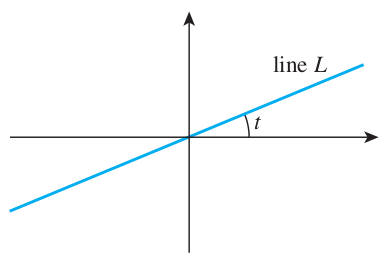
\includegraphics[scale=0.5]{../images/8.3.32.png}
\end{figure}

Alternatively, there is one equivalence class for every
possible slope: all real numbers plus “undefined.”
\end{proof}

\subsection{Exercise 33}
Let $A$ be the set of points in the rectangle with $x$ and $y$ coordinates between 0 and 1. That is, 
\[A = \{(x, y) \in \R \times \R \,|\, 0 \leq x \leq 1 \text{ and } 0 \leq y \leq 1\}.
\] 
Define a relation $R$ on $A$ as follows: For all \((x_1, y_1)\) and \((x_2, y_2)\) in $A$, 

\begin{center}
\begin{tabular}{ccccccc}
\((x_1, y_1) \,R\, (x_2, y_2) \iff\) &\((x_1, y_1)\) & = & \((x_2, y_2);\) & or \\
&\(x_1=0\) & and & \(x_2=1\) & and & \(y_1 = y_2\); & or \\
&\(x_1=1\) & and & \(x_2=0\) & and & \(y_1 = y_2\); & or \\
&\(y_1=0\) & and & \(y_2=1\) & and & \(x_1 = x_2\); & or \\
&\(y_1=1\) & and & \(y_2=0\) & and & \(x_1 = x_2\). 
\end{tabular}
\end{center}

In other words, all points along the top edge of the rectangle are related to the points along the bottom edge  
directly beneath them, and all points directly opposite each other along the left and right edges are related to  
each other. The points in the interior of the rectangle are not related to anything other than themselves. Then $R$ is 
an equivalence relation on $A$. Imagine gluing together all the points that are in the same equivalence class. Describe 
the resulting figure.

\begin{proof}
Gluing the top and bottom edges of the rectangle results in a horizontal cylinder. Then, if we also glue the left and
right circular ends of this cylinder, we get a doughnut shaped figure:

\begin{figure}[ht!]
\centering
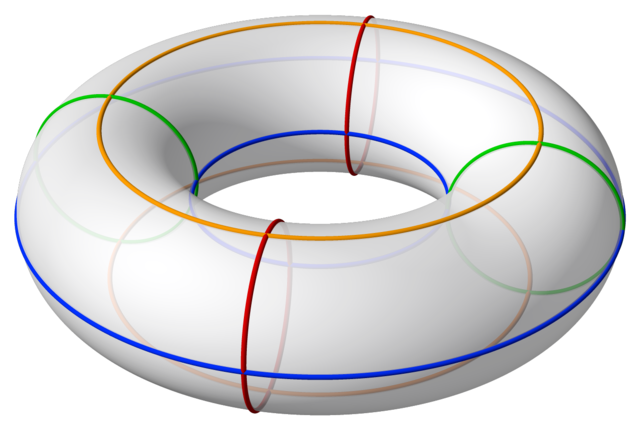
\includegraphics[scale=0.2]{../images/8.3.33.png}
\end{figure}
\end{proof}

\subsection{Exercise 34}
The documentation for the computer language Java recommends that when an “equals method” is defined for an object, it 
be an equivalence relation. That is, if $R$ is defined as follows: \(x \,R\, y \iff x.equals(y)\) for all objects in 
the class, then $R$ should be an equivalence relation. Suppose that in trying to optimize some of the mathematics 
of a graphics application, a programmer creates an object called a point, consisting of two coordinates in the plane. 
The programmer defines an equals method as follows: If $p$ and $q$ are any points, then \(p.equals(q)\) iff the 
distance from $p$ to $q$ is less than or equal to $c$ where $c$ is a small positive number that depends on the 
resolution of the computer display. Is the programmer’s equals method an equivalence relation? Justify your answer.

\begin{proof}
No. If points \(p, q\), and $r$ all lie on a straight line with $q$ in the middle, and if $p$ is $c$ units from $q$ 
and $q$ is $c$ units from $r$, then $p$ is more than $c$ units from $r$.
\end{proof}

\subsection{Exercise 35}
Find an additional representative circuit for the input/output table of Example 8.3.9.

\begin{proof}
Recall that the output table is:

\begin{center}
\arrayrulecolor{cyan}
\begin{tabular}{|cc|c|}
\hline
\multicolumn{2}{|c|}{\cy Input} & {\cy Output} \\
\hline
\(\bm{P}\) & \(\bm{Q}\) & \(\bm{R}\) \\
\hline
1 & 1 & 0 \\
\hline
1 & 0 & 0 \\
\hline
0 & 1 & 0 \\
\hline
0 & 0 & 1 \\
\hline
\end{tabular}
\arrayrulecolor{black} % change it back!
\end{center}

And two representative circuits for this table were given:

\begin{figure}[ht!]
\centering
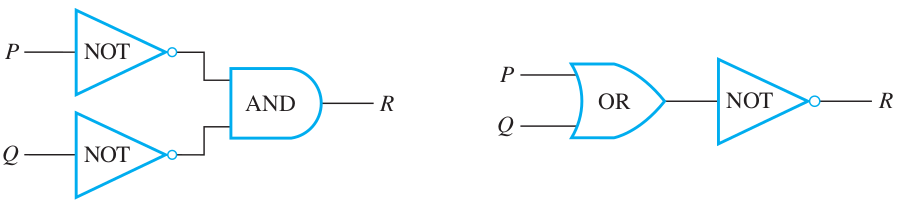
\includegraphics[scale=0.5]{../images/8.3.35.png}
\end{figure}

Here is another:

\begin{figure}[ht!]
\centering
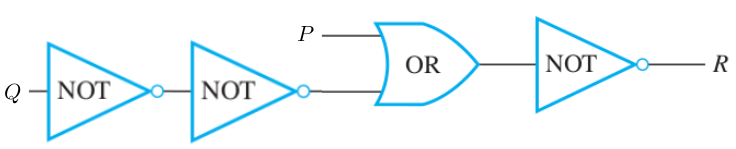
\includegraphics[scale=0.5]{../images/8.3.35.2.png}
\end{figure}
\end{proof}

{\bf \cy Let $R$ be an equivalence relation on a set $A$. Prove each of the statements in $36-41$ directly from the 
definitions of equivalence relation and equivalence class without using the results of Lemma 8.3.2, Lemma 8.3.3, or 
Theorem 8.3.4.}

\subsection{Exercise 36}
For every $a$ in $A$, \(a \in [a]\).

\begin{proof}
Suppose $R$ is an equivalence relation on a set $A$ and \(a \in A\). Because $R$ is an equivalence relation, $R$ is 
reflexive, and because $R$ is reflexive, each element of $A$ is related to itself by $R$. In particular \(a\,R\,a\). 
Hence, by definition of equivalence class, \(a \in [a]\).
\end{proof}

\subsection{Exercise 37}
For every $a$ and $b$ in $A$, if \(b \in [a]\) then \(a \,R\, b\).

\begin{proof}
Yes, by definition of \([a], b \in [a] \iff b \,R\,a\). So \(b \,R\, a\). By symmetry, \(a \,R\, b\).
\end{proof}

\subsection{Exercise 38}
For every \(a, b\), and \(c\) in \(A\), if \(b \,R\, c\) and \(c \in [a]\) then \(b \in [a]\).

\begin{proof}
Suppose $R$ is an equivalence relation on a set $A$ and \(a, b\), and $c$ are elements of $A$ with \(b \,R\, c\) and 
\(c \in [a]\). Since \(c \in [a]\), then \(c \,R\, a\) by definition of equivalence class. Now \(R\) is transitive 
because \(R\) is an equivalence relation. Thus, since \(b \,R\, c\) and \(c \,R\, a\), then \(b \,R\, a\). It follows 
that \(b \in [a]\) by definition of equivalence class.
\end{proof}

\subsection{Exercise 39}
For every $a$ and $b$ in $A$, if \([a] = [b]\) then \(a \,R\, b\).

\begin{proof}
Assume \([a] = [b]\). By Exercise 36 \(b \in [b]\), and since \([a] = [b]\) we have \(b \in [a]\). So by Exercise 
37 \(a \,R\, b\).
\end{proof}

\subsection{Exercise 40}
For every \(a, b\), and \(x\) in \(A\), if \(a \,R\, b\) and \(x \in [a]\) then \(x \in [b]\).

\begin{proof}
Suppose \(a, b\), and \(x\) are in \(A, a \,R\, b\), and \(x \in [a]\). By definition of equivalence class, 
\(x \,R\, a\). So \(x \,R\, a\) and \(a \,R\, b\), and thus, by transitivity, \(x \,R\, b\). Hence \(x \in [b]\).
\end{proof}

\subsection{Exercise 41}
For every $a$ and $b$ in $A$, if \(a \in [b]\) then \([a] = [b]\).

\begin{proof}
Assume \(x \in [a]\). Then \(x \,R\, a\) by definition of \([a]\). Since \(a \in [b]\), by Exercise 37 \(b \,R\, a\).
By symmetry, \(a \,R\, b\). Then by transitivity \(x \,R\, b\). So \(x \in [b]\) by definition of \([b]\). Thus 
\([a] \subseteq [b]\).

Assume \(x \in [b]\). Then \(x \,R\, b\) by definition of \([b]\). Since \(a \in [b]\), by Exercise 37 \(b \,R\, a\).
Then by transitivity \(x \,R\, a\). So \(x \in [a]\) by definition of \([a]\). Thus \([b] \subseteq [a]\).

So by definition of set equality \([a] = [b]\).
\end{proof}

\subsection{Exercise 42}
Let $R$ be the relation defined in Example 8.3.12: \((a,b) \,R\, (c,d) \iff ad = bc\).

\subsubsection{(a)}
Prove that $R$ is reflexive.

\begin{proof}
For all \(a \in \Z, b \in \Z - \{0\}, ab = ba\), therefore \((a,b) \,R\, (a,b)\). So $R$ is reflexive.
\end{proof}

\subsubsection{(b)}
Prove that $R$ is symmetric.

\begin{proof}
Assume \((a,b) \,R\, (c,d)\). Then \(ad = bc\). So \(bc = ad\) and thus \((c,d) \,R\, (a,b)\). So $R$ is symmetric.
\end{proof}

\subsubsection{(c)}
List four distinct elements in [(1, 3)].

\begin{proof}
One possible answer: \((2, 6), (-2, -6), (3, 9), (-3, -9)\).
\end{proof}

\subsubsection{(d)}
List four distinct elements in [(2, 5)].

\begin{proof}
One possible answer: \((4, 10), (6, 15), (8, 20), (10, 25)\).
\end{proof}

\subsection{Exercise 43}
In Example 8.3.12, define operations of addition (+) and multiplication (\(\cdot\)) as follows: For every \((a, b), 
(c, d) \in A, [(a, b)] + [(c, d)] = [(ad + bc, bd)]\) and \([(a, b)] \cdot [(c, d)] = [(ac, bd)]\).

\subsubsection{(a)}
Prove that this addition is well defined. That is, show that if \([(a, b)] = [(a', b')]\) and \([(c, d)] = [(c', 
d')]\), then \([(ad + bc, bd)] = [(a'd' + b'c', b'd')]\).

\begin{proof}
Suppose that \((a, b), (a', b'), (c, d)\), and \((c', d')\) are any elements of \(A\) such that \([(a, b)]=[(a', b')]\) 
and \([(c, d)] = [(c', d')]\). By definition of \(R, ab' = ba'\) (*) and \(cd' = dc'\) (**). We must show that 
\([(a, b)] + [(c, d)] = [(a', b')] + [(c', d')]\). By definition of the addition on \(A\), this equation is true 
if, and only if, \([(ad + bc, bd)] = [(a'd' + b'c', b'd')]\). And, by definition of the relation, this equation is 
true if, and only if, \((ad + bc)b'd' = bd(a'd' + b'c')\). After multiplying out, this becomes \(adb'd' + bcb'd' = 
bda'd' + bdb'c'\), and regrouping, turns it into \((ab')(dd') + (cd')(bb') = (ba')(dd') + (dc')(bb')\). 
Substituting the values from (*) and (**) shows that this last equation is true. 
\end{proof}

\subsubsection{(b)}
Prove that this multiplication is well defined. That is, show that if \([(a, b)] = [(a', b')]\) and \([(c, d)] = 
[(c', d')]\), then \([(ac, bd)] = [(a'c', b'd')]\).

\begin{proof}
1. Assume \([(a, b)] = [(a', b')]\) and \([(c, d)] = [(c', d')]\).

2. By 1 and the definition of equivalence classes of $R$, \((a,b) \,R\, (a',b')\) and \((c,d) \,R\, (c',d')\).

3. By 2 and definition of $R$, \(ab' = ba'\) and \(cd' = dc'\).

4. By 3, multiplying the left hand sides together and the right hand sides together, \(ab'cd' = ba'dc'\).

5. By 4 and commutativity, reorganizing, \((ac)(b'd') = (bd)(a'c')\).

6. By 5 and definition of $R$, \((ad, bc) \,R\, (a'c', b'd')\).

7. By 6 and definition of equivalence classes of $R$, \([(ad, bc)] = [(a'c', b'd')]\).
\end{proof}

\subsubsection{(c)}
Show that \([(0, 1)]\) is an identity element for addition. That is, show that for any \((a, b) \in A, [(a, b)] + [(0, 
1)] = [(0, 1)] + [(a, b)] = [(a, b)]\).

\begin{proof}
Suppose that \((a, b)\) is any element of \(A\). We must show that \([(a, b)] + [(0, 1)] = [(a, b)]\). By definition 
of the addition on \(A\), this equation is true if, and only if, \([(a \cdot 1 + b \cdot 0, b \cdot 1)]=[(a, b)]\). 
And this last equation is true because \(a \cdot 1 + b \cdot 0 = a\) and \(b \cdot 1 = b\).
\end{proof}

\subsubsection{(d)}
Find an identity element for multiplication. That is, find \((i, j)\) in \(A\) so that for every \((a, b)\) in \(A\), 
\([(a, b)] \cdot [(i, j)] = [(i, j)] \cdot [(a, b)] = [(a, b)]\).

\begin{proof}
The multiplicative identity is \((1,1)\). Indeed, by definition of multiplication on \(A\), \([(a, b)] \cdot 
[(1, 1)] = [(a \cdot 1, b \cdot 1)] = [(a,b)]\) and \([(1, 1)] \cdot [(a, b)] = [(1 \cdot a, 1 \cdot b)] = [(a,b)]\).
\end{proof}

\subsubsection{(e)}
For any \((a, b) \in A\), show that \([(-a, b)]\) is an inverse for \([(a, b)]\) for addition. That is, show that 
\([(-a, b)] + [(a, b)] = [(a, b)] + [(-a, b)] = [(0, 1)]\).

\begin{proof}
Suppose that \((a, b)\) is any element of \(A\). We must show that \([(a, b)] + [(-a, b)] = [(-a, b)] + [(a, b)] = 
[(0, 1)]\). By definition of the addition on \(A\), this equation is true if, and only if, \([(ab + b(-a), bb)] = 
[(0, 1)]\), or, equivalently, \([(0, bb)] = [(0, 1)]\). By definition of the relation, this last equation is true if, 
and only if, \(0 \cdot 1 = bb \cdot 0\), which is true.
\end{proof}

\subsubsection{(f)}
Given any \((a, b) \in A\) with \(a \neq 0\), find an inverse for \([(a, b)]\) for multiplication. That is, find 
\((c, d)\) in \(A\) so that \([(a, b)] \cdot [(c, d)] = [(c, d)] \cdot [(a, b)] = [(i, j)]\), where \([(i, j)]\) is 
the identity element you found in part (d).

\begin{proof}
Given \([(a,b)]\) we want to find \([(c,d)]\) such that \([(a,b)] \cdot [(c,d)] = [(ac,bd)] = [(1,1)]\). 

So by the definition of equivalence classes of $R$ on $A$, \((ac,bd)\) is related to \((1,1)\) by $R$, in other words 
\(ac \cdot 1 = bd \cdot 1\), or \(ac = bd\). Then let \((c,d) = (b,a)\). So \(ac = ab = ba = bd\), therefore 
\((ac,bd) \,R\, (1,1)\) and thus \([(ac,bd)] = [(1,1)]\), in other words \([(a,b)] \cdot [(c,d)] = [(1,1)]\).

Similarly we can prove that \([(c,d)] \cdot [(a,b)] = [(1,1)]\).
\end{proof}

\subsection{Exercise 44}
Let \(A = Z^+ \times Z^+\). Define a relation \(R\) on \(A\) as follows: For every \((a, b)\) and \((c, d)\) in 
\(A, (a, b) \,R\, (c, d) \iff a + d = c + b\).

\subsubsection{(a)}
Prove that $R$ is reflexive.

\begin{proof}
Let \((a, b)\) be any element of \(Z^+ \times Z^+\). We must show that \((a, b) \,R\, (a, b)\). By definition of 
$R$, this relationship holds if, and only if, \(a + b = b + a\). But this equation is true by the commutative law of 
addition for real numbers. Hence \(R\) is reflexive.
\end{proof}

\subsubsection{(b)}
Prove that $R$ is symmetric.

\begin{proof}
Assume \((a, b) \,R\, (c, d)\). Then by definition of $R$, \(a + d = c + b\). So \(c + b = a + d\). Thus 
\((c, d) \,R\, (a, b)\) by definition of $R$. So $R$ is symmetric.
\end{proof}

\subsubsection{(c)}
Prove that $R$ is transitive.

\begin{proof}
Assume \((a, b) \,R\, (c, d)\) and \((c, d)\,R\,(e, f)\). By definition of $R$, \(a + d=c + b\) and \(c + f=e + d\).
Adding the two equations we get \(a+d+c+f = c+b+e+d\). Canceling \(c+d\) on both sides we get \(a+f = e+b\), thus
\((a,b) \,R\, (e,f)\) so $R$ is transitive.
\end{proof}

\subsubsection{(d)}
List five elements in [(1, 1)].

\begin{proof}
One possible answer: (1, 1), (2, 2), (3, 3), (4, 4), (5, 5)
\end{proof}

\subsubsection{(e)}
List five elements in [(3, 1)].

\begin{proof}
One possible answer: (4, 2), (5, 3), (6, 4), (7, 5), (8, 6)
\end{proof}

\subsubsection{(f)}
List five elements in [(1, 2)].

\begin{proof}
One possible answer: (1, 2), (2, 3), (3, 4), (4, 5), (5, 6)
\end{proof}

\subsubsection{(g)}
Describe the distinct equivalence classes of $R$.

\begin{proof}
Observe that for any positive integers $a$ and $b$, the equivalence class of \((a, b)\) consists of all ordered 
pairs in \(Z^+ \times Z^+\) for which the difference between the first and second coordinates equals \(a - b\). 
Thus there is one equivalence class for each integer: positive, negative, and zero. Each positive integer \(n\) 
corresponds to the class of \((n + 1, 1)\); each negative integer \(-n\) corresponds to the class of \((1, n + 1)\); 
and zero corresponds to the class \((1, 1)\).
\end{proof}

\subsection{Exercise 45}
The following argument claims to prove that the requirement that an equivalence relation be reflexive is redundant. In 
other words, it claims to show that if a relation is symmetric and transitive, then it is reflexive. Find the 
mistake in the argument.

“Proof: Let $R$ be a relation on a set $A$ and suppose $R$ is symmetric and transitive. For any two elements $x$ and 
$y$ in $A$, if \(x \,R\, y\) then \(y \,R\, x\) since $R$ is symmetric. Thus it follows by transitivity that 
\(x \,R\, x\), and hence $R$ is reflexive.”

\begin{proof}
The conclusion \(x \,R\, x\) only follows under the assumption that \(x \,R\, y\), which has not been 
discharged from the proof. (See next exercise.)
\end{proof}

\subsection{Exercise 46}
Let $R$ be a relation on a set $A$ and suppose $R$ is symmetric and transitive. Prove the following: If for every 
$x$ in $A$ there is a $y$ in $A$ such that \(x \,R\, y\), then $R$ is an equivalence relation.

\begin{proof}
Let $R$ be a relation on a set $A$ and suppose $R$ is symmetric and transitive. Assume $x$ is any element in $A$. 
By the assumption, there exists $y$ in $A$ such that \(x \,R\, y\). Then \(y \,R\, x\) since $R$ is symmetric. Thus 
it follows by transitivity that \(x \,R\, x\), and hence $R$ is reflexive. Hence $R$ is an equivalence relation.
\end{proof}

\subsection{Exercise 47}
Refer to the quote at the beginning of this section to answer the following questions.

\subsubsection{(a)}
What is the name of the Knight’s song called?

\begin{proof}
... The name of the song is called ‘Haddocks’ Eyes.’
\end{proof}

\subsubsection{(b)}
What is the name of the Knight’s song?

\begin{proof}
The name really is ‘The Aged Aged Man.’
\end{proof}

\subsubsection{(c)}
What is the Knight’s song called?

\begin{proof}
“Ways and Means”
\end{proof}

\subsubsection{(d)}
What is the Knight’s song?

\begin{proof}
The song really is ‘A-sitting on a Gate’
\end{proof}

\subsubsection{(e)}
What is your (full, legal) name?

\begin{proof}
Spam, Egg
\end{proof}

\subsubsection{(f)}
What are you called?

\begin{proof}
Spam
\end{proof}

\subsubsection{(g)}
What are you? (Do not answer this on paper; just think about it.)

\begin{proof}
{\it ???}
\end{proof}

\section{Exercise Set 8.4}

\subsection{Exercise 1}

\subsubsection{(a)}

\begin{proof}

\end{proof}

\subsubsection{(b)}

\begin{proof}

\end{proof}

\subsection{Exercise 2}

\subsubsection{(a)}

\begin{proof}

\end{proof}

\subsubsection{(b)}

\begin{proof}

\end{proof}

\subsection{Exercise 3}

\subsubsection{(a)}

\begin{proof}

\end{proof}

\subsubsection{(b)}

\begin{proof}

\end{proof}

\subsubsection{(c)}

\begin{proof}

\end{proof}

\subsubsection{(d)}

\begin{proof}

\end{proof}

\subsubsection{(e)}

\begin{proof}

\end{proof}

\subsection{Exercise 4}

\subsubsection{(a)}

\begin{proof}

\end{proof}

\subsubsection{(b)}

\begin{proof}

\end{proof}

\subsubsection{(c)}

\begin{proof}

\end{proof}

\subsubsection{(d)}

\begin{proof}

\end{proof}

\subsubsection{(e)}

\begin{proof}

\end{proof}

\subsection{Exercise 5}

\begin{proof}

\end{proof}

\subsection{Exercise 6}

\begin{proof}

\end{proof}

\subsection{Exercise 7}

\subsubsection{(a)}

\begin{proof}

\end{proof}

\subsubsection{(b)}

\begin{proof}

\end{proof}

\subsubsection{(c)}

\begin{proof}

\end{proof}

\subsubsection{(d)}

\begin{proof}

\end{proof}

\subsubsection{(e)}

\begin{proof}

\end{proof}

\subsection{Exercise 8}

\subsubsection{(a)}

\begin{proof}

\end{proof}

\subsubsection{(b)}

\begin{proof}

\end{proof}

\subsubsection{(c)}

\begin{proof}

\end{proof}

\subsubsection{(d)}

\begin{proof}

\end{proof}

\subsubsection{(e)}

\begin{proof}

\end{proof}

\subsection{Exercise 9}

\subsubsection{(a)}

\begin{proof}

\end{proof}

\subsubsection{(b)}

\begin{proof}

\end{proof}

\subsection{Exercise 10}

\begin{proof}

\end{proof}

\subsection{Exercise 11}

\begin{proof}

\end{proof}

\subsection{Exercise 12}

\subsubsection{(a)}

\begin{proof}

\end{proof}

\subsubsection{(b)}

\begin{proof}

\end{proof}

\subsection{Exercise 13}

\subsubsection{(a)}

\begin{proof}

\end{proof}

\subsubsection{(b)}

\begin{proof}

\end{proof}

\subsection{Exercise 14}

\begin{proof}

\end{proof}

\subsection{Exercise 15}

\begin{proof}

\end{proof}

\subsection{Exercise 16}

\begin{proof}

\end{proof}

\subsection{Exercise 17}

\begin{proof}

\end{proof}

\subsection{Exercise 18}

\begin{proof}

\end{proof}

\subsection{Exercise 19}

\begin{proof}

\end{proof}

\subsection{Exercise 20}

\begin{proof}

\end{proof}

\subsection{Exercise 21}

\begin{proof}

\end{proof}

\subsection{Exercise 22}

\begin{proof}

\end{proof}

\subsection{Exercise 23}

\begin{proof}

\end{proof}

\subsection{Exercise 24}

\begin{proof}

\end{proof}

\subsection{Exercise 25}

\begin{proof}

\end{proof}

\subsection{Exercise 26}

\begin{proof}

\end{proof}

\subsection{Exercise 27}

\begin{proof}

\end{proof}

\subsection{Exercise 28}

\begin{proof}

\end{proof}

\subsection{Exercise 29}

\begin{proof}

\end{proof}

\subsection{Exercise 30}

\begin{proof}

\end{proof}

\subsection{Exercise 31}

\subsubsection{(a)}

\begin{proof}

\end{proof}

\subsubsection{(b)}

\begin{proof}

\end{proof}

\subsubsection{(c)}

\begin{proof}

\end{proof}

\subsection{Exercise 32}

\subsubsection{(a)}

\begin{proof}

\end{proof}

\subsubsection{(b)}

\begin{proof}

\end{proof}

\subsection{Exercise 33}

\begin{proof}

\end{proof}

\subsection{Exercise 34}

\begin{proof}

\end{proof}

\subsection{Exercise 35}

\begin{proof}

\end{proof}

\subsection{Exercise 36}

\begin{proof}

\end{proof}

\subsection{Exercise 37}

\begin{proof}

\end{proof}

\subsection{Exercise 38}

\begin{proof}

\end{proof}

\subsection{Exercise 39}

\begin{proof}

\end{proof}

\subsection{Exercise 40}

\begin{proof}

\end{proof}

\subsection{Exercise 41}

\subsubsection{(a)}

\begin{proof}

\end{proof}

\subsubsection{(b)}

\begin{proof}

\end{proof}

\subsection{Exercise 42}

\begin{proof}

\end{proof}

\subsection{Exercise 43}

\begin{proof}

\end{proof}

\section{Exercise Set 8.5}

\subsection{Exercise 1}

\subsubsection{(a)}

\begin{proof}

\end{proof}

\subsubsection{(b)}

\begin{proof}

\end{proof}

\subsubsection{(c)}

\begin{proof}

\end{proof}

\subsubsection{(d)}

\begin{proof}

\end{proof}

\subsection{Exercise 2}

\begin{proof}

\end{proof}

\subsection{Exercise 3}

\begin{proof}

\end{proof}

\subsection{Exercise 4}

\begin{proof}

\end{proof}

\subsection{Exercise 5}

\begin{proof}

\end{proof}

\subsection{Exercise 6}

\begin{proof}

\end{proof}

\subsection{Exercise 7}

\begin{proof}

\end{proof}

\subsection{Exercise 8}

\begin{proof}

\end{proof}

\subsection{Exercise 9}

\begin{proof}

\end{proof}

\subsection{Exercise 10}

\begin{proof}

\end{proof}

\subsection{Exercise 11}

\subsubsection{(a)}

\begin{proof}

\end{proof}

\subsubsection{(b)}

\begin{proof}

\end{proof}

\subsubsection{(c)}

\begin{proof}

\end{proof}

\subsubsection{(d)}

\begin{proof}

\end{proof}

\subsubsection{(e)}

\begin{proof}

\end{proof}

\subsubsection{(f)}

\begin{proof}

\end{proof}

\subsubsection{(g)}

\begin{proof}

\end{proof}

\subsection{Exercise 12}

\begin{proof}

\end{proof}

\subsection{Exercise 13}

\begin{proof}

\end{proof}

\subsection{Exercise 14}

\subsubsection{(a)}

\begin{proof}

\end{proof}

\subsubsection{(b)}

\begin{proof}

\end{proof}

\subsection{Exercise 15}

\begin{proof}

\end{proof}

\subsection{Exercise 16}

\subsubsection{(a)}

\begin{proof}

\end{proof}

\subsubsection{(b)}

\begin{proof}

\end{proof}

\subsection{Exercise 17}

\begin{proof}

\end{proof}

\subsection{Exercise 18}

\begin{proof}

\end{proof}

\subsection{Exercise 19}

\begin{proof}

\end{proof}

\subsection{Exercise 20}

\begin{proof}

\end{proof}

\subsection{Exercise 21}

\subsubsection{(a)}

\begin{proof}

\end{proof}

\subsubsection{(b)}

\begin{proof}

\end{proof}

\subsection{Exercise 22}

\begin{proof}

\end{proof}

\subsection{Exercise 23}

\begin{proof}

\end{proof}

\subsection{Exercise 24}

\begin{proof}

\end{proof}

\subsection{Exercise 25}

\begin{proof}

\end{proof}

\subsection{Exercise 26}

\begin{proof}

\end{proof}

\subsection{Exercise 27}

\begin{proof}

\end{proof}

\subsection{Exercise 28}

\begin{proof}

\end{proof}

\subsection{Exercise 29}

\begin{proof}

\end{proof}

\subsection{Exercise 30}

\subsubsection{(a)}

\begin{proof}

\end{proof}

\subsubsection{(b)}

\begin{proof}

\end{proof}

\subsubsection{(c)}

\begin{proof}

\end{proof}

\subsubsection{(d)}

\begin{proof}

\end{proof}

\subsection{Exercise 31}

\begin{proof}

\end{proof}

\subsection{Exercise 32}

\begin{proof}

\end{proof}

\subsection{Exercise 33}

\begin{proof}

\end{proof}

\subsection{Exercise 34}

\begin{proof}

\end{proof}

\subsection{Exercise 35}

\begin{proof}

\end{proof}

\subsection{Exercise 36}

\begin{proof}

\end{proof}

\subsection{Exercise 37}

\begin{proof}

\end{proof}

\subsection{Exercise 38}

\begin{proof}

\end{proof}

\subsection{Exercise 39}

\begin{proof}

\end{proof}

\subsection{Exercise 40}

\subsubsection{(a)}

\begin{proof}

\end{proof}

\subsubsection{(b)}

\begin{proof}

\end{proof}

\subsection{Exercise 41}

\subsubsection{(a)}

\begin{proof}

\end{proof}

\subsubsection{(b)}

\begin{proof}

\end{proof}

\subsection{Exercise 42}

\begin{proof}

\end{proof}

\subsection{Exercise 43}

\begin{proof}

\end{proof}

\subsection{Exercise 44}

\begin{proof}

\end{proof}

\subsection{Exercise 45}

\begin{proof}

\end{proof}

\subsection{Exercise 46}

\begin{proof}

\end{proof}

\subsection{Exercise 47}

\begin{proof}

\end{proof}

\subsection{Exercise 48}

\begin{proof}

\end{proof}

\subsection{Exercise 49}

\subsubsection{(a)}

\begin{proof}

\end{proof}

\subsubsection{(b)}

\begin{proof}

\end{proof}

\subsection{Exercise 50}

\subsubsection{(a)}

\begin{proof}

\end{proof}

\subsubsection{(b)}

\begin{proof}

\end{proof}

\subsection{Exercise 51}

\subsubsection{(a)}

\begin{proof}

\end{proof}

\subsubsection{(b)}

\begin{proof}

\end{proof}

\end{document}
